\documentclass[tikz]{standalone}
\usetikzlibrary{trees}
\begin{document}
\tikzstyle{every node}=[shape=rectangle,rounded corners,draw=black,thick,top color=white,bottom color=blue!20,anchor=west]
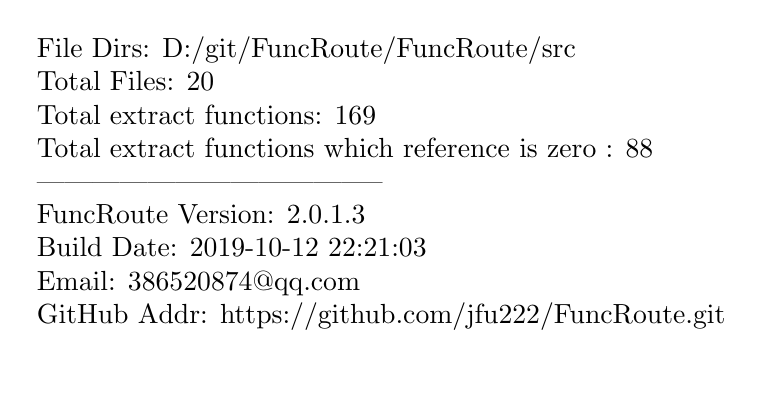
\begin{tikzpicture}
\node [align=left] {File Dirs: D:/git/FuncRoute/FuncRoute/src\\Total Files: 20\\Total extract functions: 169\\Total extract functions which reference is zero : 88\\--------------------------------------\\FuncRoute Version: 2.0.1.3\\Build Date: 2019-10-12 22:21:03\\Email: 386520874@qq.com\\GitHub Addr: https://github.com/jfu222/FuncRoute.git\\};
\end{tikzpicture}
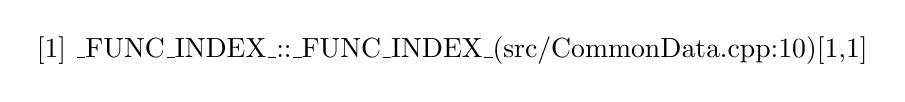
\begin{tikzpicture}[grow via three points={one child at (0.5,-0.7) and two children at (0.5,-0.7) and (0.5,-1.4)}, edge from parent path={(\tikzparentnode.south) |- (\tikzchildnode.west)}]
\node {[1] \_FUNC\_INDEX\_::\_FUNC\_INDEX\_(src/CommonData.cpp:10)[1,1]}
;
\end{tikzpicture}

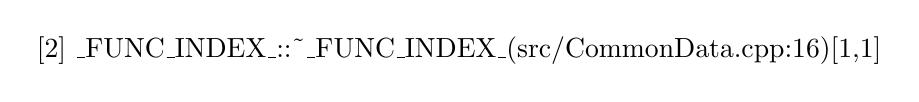
\begin{tikzpicture}[grow via three points={one child at (0.5,-0.7) and two children at (0.5,-0.7) and (0.5,-1.4)}, edge from parent path={(\tikzparentnode.south) |- (\tikzchildnode.west)}]
\node {[2] \_FUNC\_INDEX\_::\~{}\_FUNC\_INDEX\_(src/CommonData.cpp:16)[1,1]}
;
\end{tikzpicture}

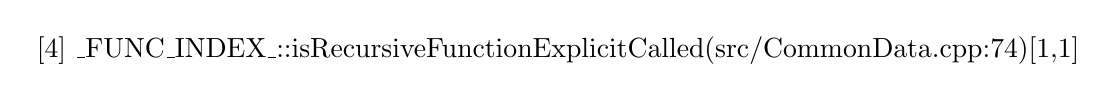
\begin{tikzpicture}[grow via three points={one child at (0.5,-0.7) and two children at (0.5,-0.7) and (0.5,-1.4)}, edge from parent path={(\tikzparentnode.south) |- (\tikzchildnode.west)}]
\node {[4] \_FUNC\_INDEX\_::isRecursiveFunctionExplicitCalled(src/CommonData.cpp:74)[1,1]}
;
\end{tikzpicture}

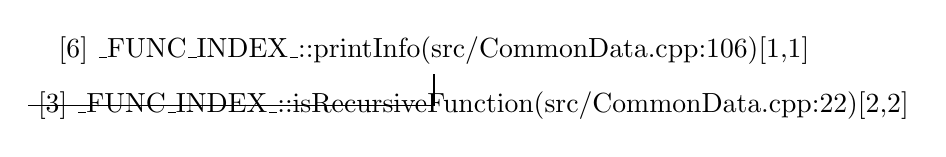
\begin{tikzpicture}[grow via three points={one child at (0.5,-0.7) and two children at (0.5,-0.7) and (0.5,-1.4)}, edge from parent path={(\tikzparentnode.south) |- (\tikzchildnode.west)}]
\node {[6] \_FUNC\_INDEX\_::printInfo(src/CommonData.cpp:106)[1,1]}
    child { node {[3] \_FUNC\_INDEX\_::isRecursiveFunction(src/CommonData.cpp:22)[2,2]} 
        }
;
\end{tikzpicture}

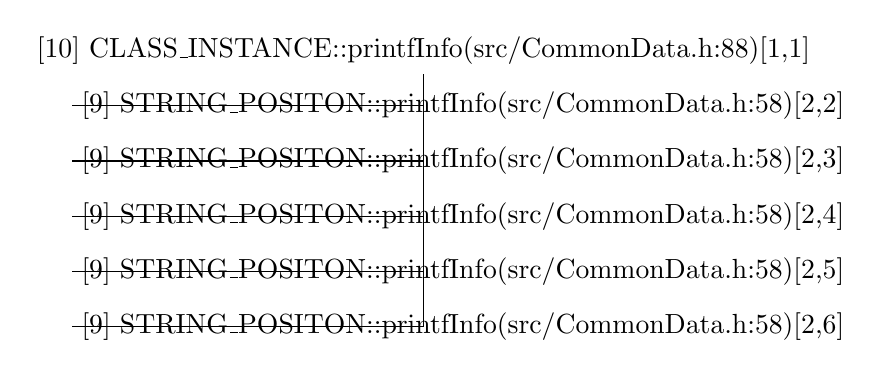
\begin{tikzpicture}[grow via three points={one child at (0.5,-0.7) and two children at (0.5,-0.7) and (0.5,-1.4)}, edge from parent path={(\tikzparentnode.south) |- (\tikzchildnode.west)}]
\node {[10] CLASS\_INSTANCE::printfInfo(src/CommonData.h:88)[1,1]}
    child { node {[9] STRING\_POSITON::printfInfo(src/CommonData.h:58)[2,2]} 
        }
    child { node {[9] STRING\_POSITON::printfInfo(src/CommonData.h:58)[2,3]} 
        }
    child { node {[9] STRING\_POSITON::printfInfo(src/CommonData.h:58)[2,4]} 
        }
    child { node {[9] STRING\_POSITON::printfInfo(src/CommonData.h:58)[2,5]} 
        }
    child { node {[9] STRING\_POSITON::printfInfo(src/CommonData.h:58)[2,6]} 
        }
;
\end{tikzpicture}

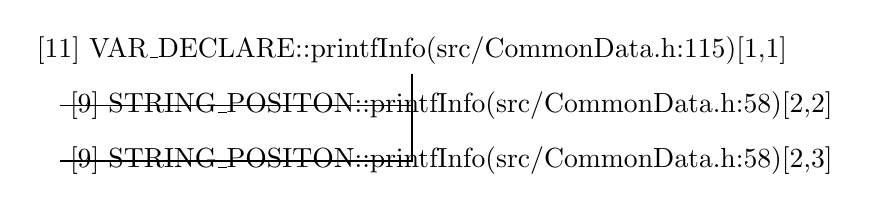
\begin{tikzpicture}[grow via three points={one child at (0.5,-0.7) and two children at (0.5,-0.7) and (0.5,-1.4)}, edge from parent path={(\tikzparentnode.south) |- (\tikzchildnode.west)}]
\node {[11] VAR\_DECLARE::printfInfo(src/CommonData.h:115)[1,1]}
    child { node {[9] STRING\_POSITON::printfInfo(src/CommonData.h:58)[2,2]} 
        }
    child { node {[9] STRING\_POSITON::printfInfo(src/CommonData.h:58)[2,3]} 
        }
;
\end{tikzpicture}

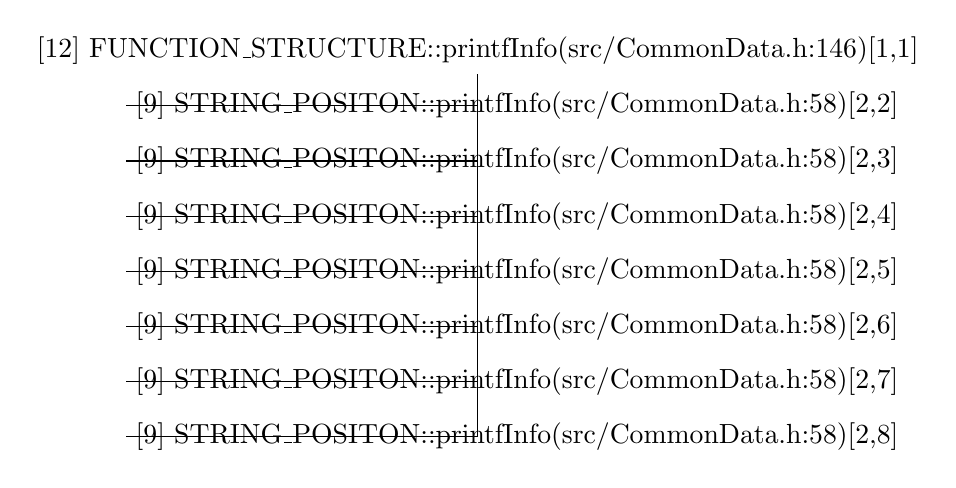
\begin{tikzpicture}[grow via three points={one child at (0.5,-0.7) and two children at (0.5,-0.7) and (0.5,-1.4)}, edge from parent path={(\tikzparentnode.south) |- (\tikzchildnode.west)}]
\node {[12] FUNCTION\_STRUCTURE::printfInfo(src/CommonData.h:146)[1,1]}
    child { node {[9] STRING\_POSITON::printfInfo(src/CommonData.h:58)[2,2]} 
        }
    child { node {[9] STRING\_POSITON::printfInfo(src/CommonData.h:58)[2,3]} 
        }
    child { node {[9] STRING\_POSITON::printfInfo(src/CommonData.h:58)[2,4]} 
        }
    child { node {[9] STRING\_POSITON::printfInfo(src/CommonData.h:58)[2,5]} 
        }
    child { node {[9] STRING\_POSITON::printfInfo(src/CommonData.h:58)[2,6]} 
        }
    child { node {[9] STRING\_POSITON::printfInfo(src/CommonData.h:58)[2,7]} 
        }
    child { node {[9] STRING\_POSITON::printfInfo(src/CommonData.h:58)[2,8]} 
        }
;
\end{tikzpicture}

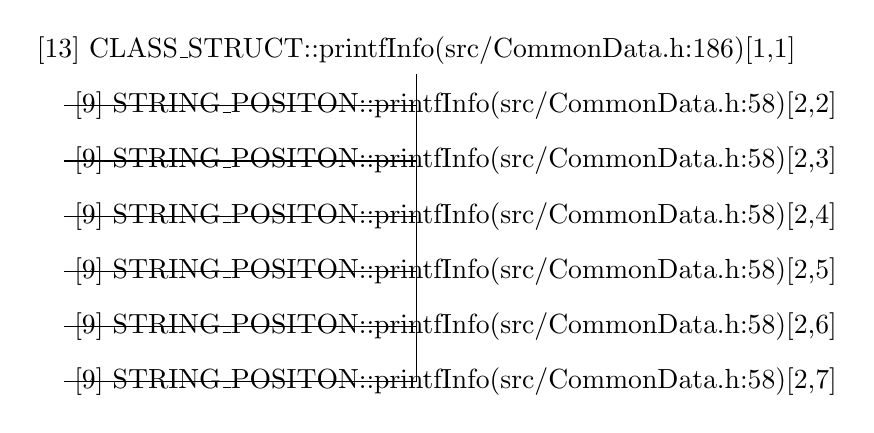
\begin{tikzpicture}[grow via three points={one child at (0.5,-0.7) and two children at (0.5,-0.7) and (0.5,-1.4)}, edge from parent path={(\tikzparentnode.south) |- (\tikzchildnode.west)}]
\node {[13] CLASS\_STRUCT::printfInfo(src/CommonData.h:186)[1,1]}
    child { node {[9] STRING\_POSITON::printfInfo(src/CommonData.h:58)[2,2]} 
        }
    child { node {[9] STRING\_POSITON::printfInfo(src/CommonData.h:58)[2,3]} 
        }
    child { node {[9] STRING\_POSITON::printfInfo(src/CommonData.h:58)[2,4]} 
        }
    child { node {[9] STRING\_POSITON::printfInfo(src/CommonData.h:58)[2,5]} 
        }
    child { node {[9] STRING\_POSITON::printfInfo(src/CommonData.h:58)[2,6]} 
        }
    child { node {[9] STRING\_POSITON::printfInfo(src/CommonData.h:58)[2,7]} 
        }
;
\end{tikzpicture}

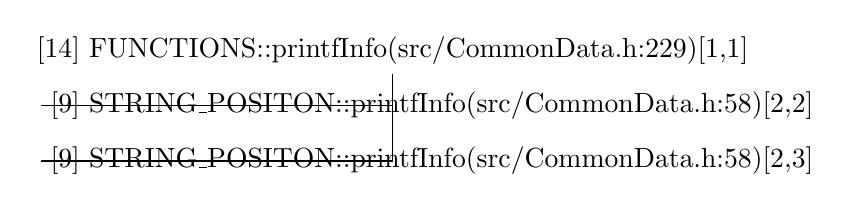
\begin{tikzpicture}[grow via three points={one child at (0.5,-0.7) and two children at (0.5,-0.7) and (0.5,-1.4)}, edge from parent path={(\tikzparentnode.south) |- (\tikzchildnode.west)}]
\node {[14] FUNCTIONS::printfInfo(src/CommonData.h:229)[1,1]}
    child { node {[9] STRING\_POSITON::printfInfo(src/CommonData.h:58)[2,2]} 
        }
    child { node {[9] STRING\_POSITON::printfInfo(src/CommonData.h:58)[2,3]} 
        }
;
\end{tikzpicture}

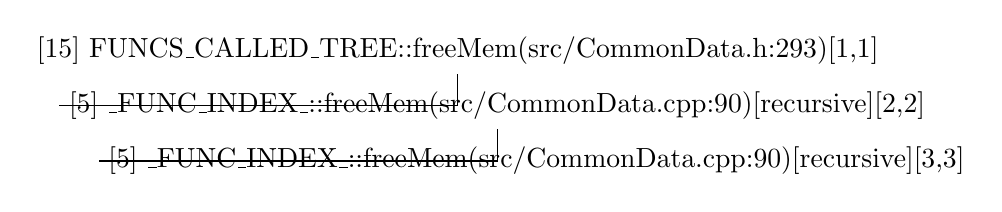
\begin{tikzpicture}[grow via three points={one child at (0.5,-0.7) and two children at (0.5,-0.7) and (0.5,-1.4)}, edge from parent path={(\tikzparentnode.south) |- (\tikzchildnode.west)}]
\node {[15] FUNCS\_CALLED\_TREE::freeMem(src/CommonData.h:293)[1,1]}
    child { node {[5] \_FUNC\_INDEX\_::freeMem(src/CommonData.cpp:90)[recursive][2,2]} 
        child { node {[5] \_FUNC\_INDEX\_::freeMem(src/CommonData.cpp:90)[recursive][3,3]} 
            }
        }
        child [missing] {}
;
\end{tikzpicture}

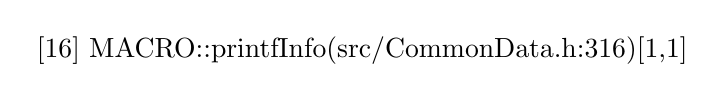
\begin{tikzpicture}[grow via three points={one child at (0.5,-0.7) and two children at (0.5,-0.7) and (0.5,-1.4)}, edge from parent path={(\tikzparentnode.south) |- (\tikzchildnode.west)}]
\node {[16] MACRO::printfInfo(src/CommonData.h:316)[1,1]}
;
\end{tikzpicture}

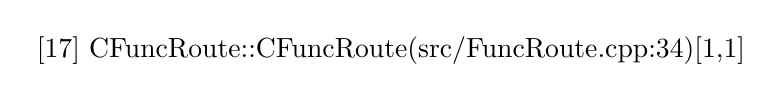
\begin{tikzpicture}[grow via three points={one child at (0.5,-0.7) and two children at (0.5,-0.7) and (0.5,-1.4)}, edge from parent path={(\tikzparentnode.south) |- (\tikzchildnode.west)}]
\node {[17] CFuncRoute::CFuncRoute(src/FuncRoute.cpp:34)[1,1]}
;
\end{tikzpicture}

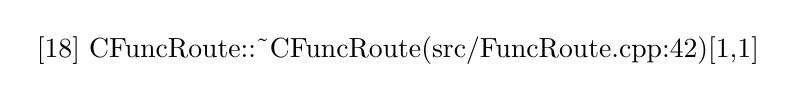
\begin{tikzpicture}[grow via three points={one child at (0.5,-0.7) and two children at (0.5,-0.7) and (0.5,-1.4)}, edge from parent path={(\tikzparentnode.south) |- (\tikzchildnode.west)}]
\node {[18] CFuncRoute::\~{}CFuncRoute(src/FuncRoute.cpp:42)[1,1]}
;
\end{tikzpicture}

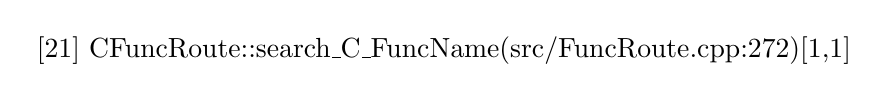
\begin{tikzpicture}[grow via three points={one child at (0.5,-0.7) and two children at (0.5,-0.7) and (0.5,-1.4)}, edge from parent path={(\tikzparentnode.south) |- (\tikzchildnode.west)}]
\node {[21] CFuncRoute::search\_C\_FuncName(src/FuncRoute.cpp:272)[1,1]}
;
\end{tikzpicture}

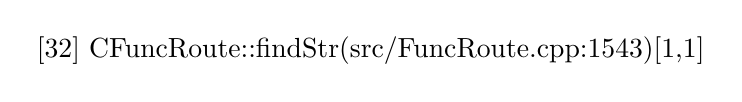
\begin{tikzpicture}[grow via three points={one child at (0.5,-0.7) and two children at (0.5,-0.7) and (0.5,-1.4)}, edge from parent path={(\tikzparentnode.south) |- (\tikzchildnode.west)}]
\node {[32] CFuncRoute::findStr(src/FuncRoute.cpp:1543)[1,1]}
;
\end{tikzpicture}

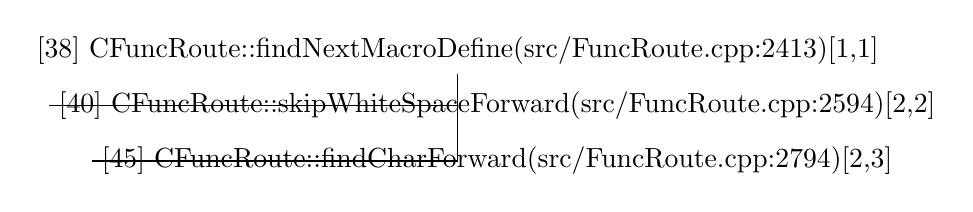
\begin{tikzpicture}[grow via three points={one child at (0.5,-0.7) and two children at (0.5,-0.7) and (0.5,-1.4)}, edge from parent path={(\tikzparentnode.south) |- (\tikzchildnode.west)}]
\node {[38] CFuncRoute::findNextMacroDefine(src/FuncRoute.cpp:2413)[1,1]}
    child { node {[40] CFuncRoute::skipWhiteSpaceForward(src/FuncRoute.cpp:2594)[2,2]} 
        }
    child { node {[45] CFuncRoute::findCharForward(src/FuncRoute.cpp:2794)[2,3]} 
        }
;
\end{tikzpicture}

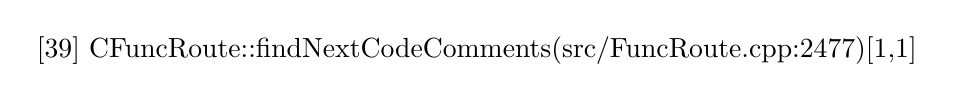
\begin{tikzpicture}[grow via three points={one child at (0.5,-0.7) and two children at (0.5,-0.7) and (0.5,-1.4)}, edge from parent path={(\tikzparentnode.south) |- (\tikzchildnode.west)}]
\node {[39] CFuncRoute::findNextCodeComments(src/FuncRoute.cpp:2477)[1,1]}
;
\end{tikzpicture}

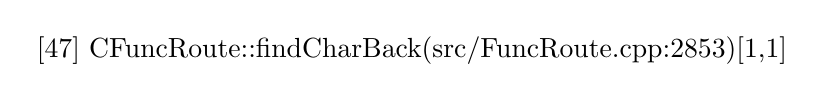
\begin{tikzpicture}[grow via three points={one child at (0.5,-0.7) and two children at (0.5,-0.7) and (0.5,-1.4)}, edge from parent path={(\tikzparentnode.south) |- (\tikzchildnode.west)}]
\node {[47] CFuncRoute::findCharBack(src/FuncRoute.cpp:2853)[1,1]}
;
\end{tikzpicture}

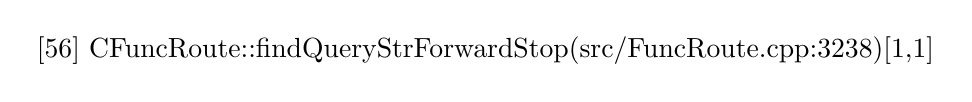
\begin{tikzpicture}[grow via three points={one child at (0.5,-0.7) and two children at (0.5,-0.7) and (0.5,-1.4)}, edge from parent path={(\tikzparentnode.south) |- (\tikzchildnode.west)}]
\node {[56] CFuncRoute::findQueryStrForwardStop(src/FuncRoute.cpp:3238)[1,1]}
;
\end{tikzpicture}

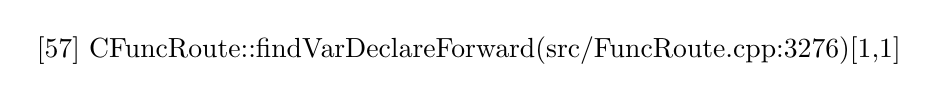
\begin{tikzpicture}[grow via three points={one child at (0.5,-0.7) and two children at (0.5,-0.7) and (0.5,-1.4)}, edge from parent path={(\tikzparentnode.south) |- (\tikzchildnode.west)}]
\node {[57] CFuncRoute::findVarDeclareForward(src/FuncRoute.cpp:3276)[1,1]}
;
\end{tikzpicture}

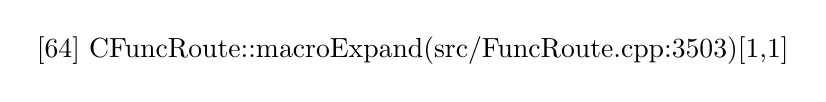
\begin{tikzpicture}[grow via three points={one child at (0.5,-0.7) and two children at (0.5,-0.7) and (0.5,-1.4)}, edge from parent path={(\tikzparentnode.south) |- (\tikzchildnode.west)}]
\node {[64] CFuncRoute::macroExpand(src/FuncRoute.cpp:3503)[1,1]}
;
\end{tikzpicture}

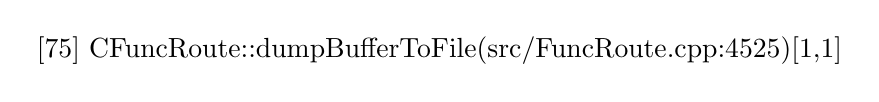
\begin{tikzpicture}[grow via three points={one child at (0.5,-0.7) and two children at (0.5,-0.7) and (0.5,-1.4)}, edge from parent path={(\tikzparentnode.south) |- (\tikzchildnode.west)}]
\node {[75] CFuncRoute::dumpBufferToFile(src/FuncRoute.cpp:4525)[1,1]}
;
\end{tikzpicture}

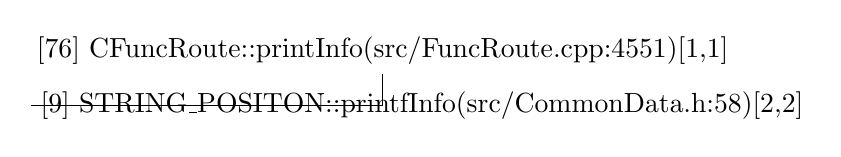
\begin{tikzpicture}[grow via three points={one child at (0.5,-0.7) and two children at (0.5,-0.7) and (0.5,-1.4)}, edge from parent path={(\tikzparentnode.south) |- (\tikzchildnode.west)}]
\node {[76] CFuncRoute::printInfo(src/FuncRoute.cpp:4551)[1,1]}
    child { node {[9] STRING\_POSITON::printfInfo(src/CommonData.h:58)[2,2]} 
        }
;
\end{tikzpicture}

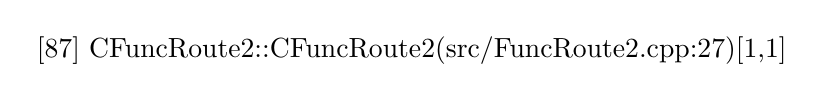
\begin{tikzpicture}[grow via three points={one child at (0.5,-0.7) and two children at (0.5,-0.7) and (0.5,-1.4)}, edge from parent path={(\tikzparentnode.south) |- (\tikzchildnode.west)}]
\node {[87] CFuncRoute2::CFuncRoute2(src/FuncRoute2.cpp:27)[1,1]}
;
\end{tikzpicture}

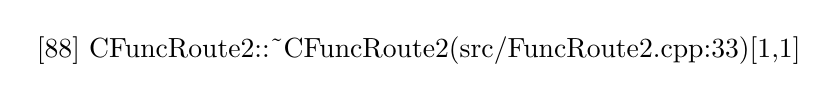
\begin{tikzpicture}[grow via three points={one child at (0.5,-0.7) and two children at (0.5,-0.7) and (0.5,-1.4)}, edge from parent path={(\tikzparentnode.south) |- (\tikzchildnode.west)}]
\node {[88] CFuncRoute2::\~{}CFuncRoute2(src/FuncRoute2.cpp:33)[1,1]}
;
\end{tikzpicture}

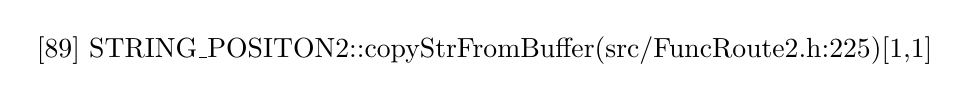
\begin{tikzpicture}[grow via three points={one child at (0.5,-0.7) and two children at (0.5,-0.7) and (0.5,-1.4)}, edge from parent path={(\tikzparentnode.south) |- (\tikzchildnode.west)}]
\node {[89] STRING\_POSITON2::copyStrFromBuffer(src/FuncRoute2.h:225)[1,1]}
;
\end{tikzpicture}

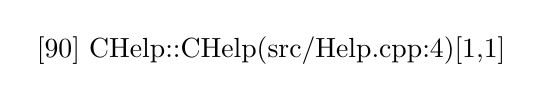
\begin{tikzpicture}[grow via three points={one child at (0.5,-0.7) and two children at (0.5,-0.7) and (0.5,-1.4)}, edge from parent path={(\tikzparentnode.south) |- (\tikzchildnode.west)}]
\node {[90] CHelp::CHelp(src/Help.cpp:4)[1,1]}
;
\end{tikzpicture}

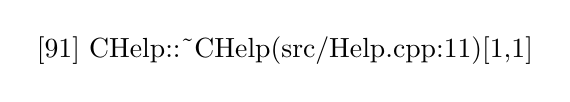
\begin{tikzpicture}[grow via three points={one child at (0.5,-0.7) and two children at (0.5,-0.7) and (0.5,-1.4)}, edge from parent path={(\tikzparentnode.south) |- (\tikzchildnode.west)}]
\node {[91] CHelp::\~{}CHelp(src/Help.cpp:11)[1,1]}
;
\end{tikzpicture}

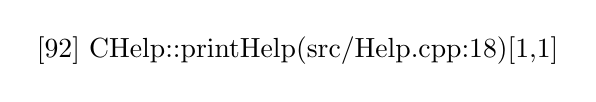
\begin{tikzpicture}[grow via three points={one child at (0.5,-0.7) and two children at (0.5,-0.7) and (0.5,-1.4)}, edge from parent path={(\tikzparentnode.south) |- (\tikzchildnode.west)}]
\node {[92] CHelp::printHelp(src/Help.cpp:18)[1,1]}
;
\end{tikzpicture}

\begin{tikzpicture}[grow via three points={one child at (0.5,-0.7) and two children at (0.5,-0.7) and (0.5,-1.4)}, edge from parent path={(\tikzparentnode.south) |- (\tikzchildnode.west)}]
\node {[94] main(src/main.cpp:27)[1,1]}
    child { node {[93] printHelp(src/main.cpp:6)[2,2]} 
        }
    child { node {[19] CFuncRoute::splitDirsBySemicolon(src/FuncRoute.cpp:48)[2,3]} 
        }
    child { node {[19] CFuncRoute::splitDirsBySemicolon(src/FuncRoute.cpp:48)[2,4]} 
        }
    child { node {[20] CFuncRoute::findAllFunctionsName(src/FuncRoute.cpp:93)[2,5]} 
        child { node {[121] get\_nested\_dir\_files(win32/shared\_library\_win32.cpp:135)[recursive][3,6]} 
            child { node {[121] get\_nested\_dir\_files(win32/shared\_library\_win32.cpp:135)[recursive][4,7]} 
                }
            }
            child [missing] {}
        child { node {[121] get\_nested\_dir\_files(win32/shared\_library\_win32.cpp:135)[recursive][3,8]} 
            }
        child { node {[33] CFuncRoute::findAllMacros(src/FuncRoute.cpp:1569)[3,9]} 
            child { node {[26] CFuncRoute::replaceAllCodeCommentsBySpace(src/FuncRoute.cpp:1076)[4,10]} 
                child { node {[27] CFuncRoute::findCurLineStartAndEndPos(src/FuncRoute.cpp:1181)[5,11]} 
                    }
                child { node {[28] CFuncRoute::isBetweenInDoubleQuotes(src/FuncRoute.cpp:1223)[5,12]} 
                    child { node {[45] CFuncRoute::findCharForward(src/FuncRoute.cpp:2794)[6,13]} 
                        }
                    child { node {[45] CFuncRoute::findCharForward(src/FuncRoute.cpp:2794)[6,14]} 
                        }
                    }
                    child [missing] {}
                    child [missing] {}
                child { node {[27] CFuncRoute::findCurLineStartAndEndPos(src/FuncRoute.cpp:1181)[5,15]} 
                    }
                child { node {[28] CFuncRoute::isBetweenInDoubleQuotes(src/FuncRoute.cpp:1223)[5,16]} 
                    child { node {[45] CFuncRoute::findCharForward(src/FuncRoute.cpp:2794)[6,17]} 
                        }
                    child { node {[45] CFuncRoute::findCharForward(src/FuncRoute.cpp:2794)[6,18]} 
                        }
                    }
                    child [missing] {}
                    child [missing] {}
                    }
                    child [missing] {}
                    child [missing] {}
                    child [missing] {}
                    child [missing] {}
                    child [missing] {}
                    child [missing] {}
                    child [missing] {}
                    child [missing] {}
                    }
                    child [missing] {}
                    child [missing] {}
                    child [missing] {}
                    child [missing] {}
                    child [missing] {}
                    child [missing] {}
                    child [missing] {}
                    child [missing] {}
                    child [missing] {}
        child { node {[166] time\_get\_tick(win32/timer\_win32.cpp:6)[3,19]} 
            }
        child { node {[125] print\_date\_time(win32/shared\_library\_win32.cpp:218)[3,20]} 
            }
        child { node {[22] CFuncRoute::search\_CPP\_FuncName(src/FuncRoute.cpp:280)[3,21]} 
            child { node {[26] CFuncRoute::replaceAllCodeCommentsBySpace(src/FuncRoute.cpp:1076)[4,22]} 
                child { node {[27] CFuncRoute::findCurLineStartAndEndPos(src/FuncRoute.cpp:1181)[5,23]} 
                    }
                child { node {[28] CFuncRoute::isBetweenInDoubleQuotes(src/FuncRoute.cpp:1223)[5,24]} 
                    child { node {[45] CFuncRoute::findCharForward(src/FuncRoute.cpp:2794)[6,25]} 
                        }
                    child { node {[45] CFuncRoute::findCharForward(src/FuncRoute.cpp:2794)[6,26]} 
                        }
                    }
                    child [missing] {}
                    child [missing] {}
                child { node {[27] CFuncRoute::findCurLineStartAndEndPos(src/FuncRoute.cpp:1181)[5,27]} 
                    }
                child { node {[28] CFuncRoute::isBetweenInDoubleQuotes(src/FuncRoute.cpp:1223)[5,28]} 
                    child { node {[45] CFuncRoute::findCharForward(src/FuncRoute.cpp:2794)[6,29]} 
                        }
                    child { node {[45] CFuncRoute::findCharForward(src/FuncRoute.cpp:2794)[6,30]} 
                        }
                    }
                    child [missing] {}
                    child [missing] {}
                    }
                    child [missing] {}
                    child [missing] {}
                    child [missing] {}
                    child [missing] {}
                    child [missing] {}
                    child [missing] {}
                    child [missing] {}
                    child [missing] {}
            child { node {[30] CFuncRoute::replaceAllStrBySpace(src/FuncRoute.cpp:1413)[4,31]} 
                child { node {[27] CFuncRoute::findCurLineStartAndEndPos(src/FuncRoute.cpp:1181)[5,32]} 
                    }
                child { node {[28] CFuncRoute::isBetweenInDoubleQuotes(src/FuncRoute.cpp:1223)[5,33]} 
                    child { node {[45] CFuncRoute::findCharForward(src/FuncRoute.cpp:2794)[6,34]} 
                        }
                    child { node {[45] CFuncRoute::findCharForward(src/FuncRoute.cpp:2794)[6,35]} 
                        }
                    }
                    child [missing] {}
                    child [missing] {}
                child { node {[27] CFuncRoute::findCurLineStartAndEndPos(src/FuncRoute.cpp:1181)[5,36]} 
                    }
                child { node {[29] CFuncRoute::isBetweenInSingleQuotes(src/FuncRoute.cpp:1318)[5,37]} 
                    child { node {[45] CFuncRoute::findCharForward(src/FuncRoute.cpp:2794)[6,38]} 
                        }
                    child { node {[45] CFuncRoute::findCharForward(src/FuncRoute.cpp:2794)[6,39]} 
                        }
                    }
                    child [missing] {}
                    child [missing] {}
                    }
                    child [missing] {}
                    child [missing] {}
                    child [missing] {}
                    child [missing] {}
                    child [missing] {}
                    child [missing] {}
                    child [missing] {}
                    child [missing] {}
            child { node {[31] CFuncRoute::replaceAllMacroDefineStrBySpace(src/FuncRoute.cpp:1484)[4,40]} 
                child { node {[40] CFuncRoute::skipWhiteSpaceForward(src/FuncRoute.cpp:2594)[5,41]} 
                    }
                child { node {[45] CFuncRoute::findCharForward(src/FuncRoute.cpp:2794)[5,42]} 
                    }
                }
                child [missing] {}
                child [missing] {}
            child { node {[34] CFuncRoute::findAllClassAndStructDeclare(src/FuncRoute.cpp:1813)[4,43]} 
                child { node {[60] CFuncRoute::isValidVarChar(src/FuncRoute.cpp:3409)[5,44]} 
                    }
                child { node {[61] CFuncRoute::isWhiteSpace(src/FuncRoute.cpp:3423)[5,45]} 
                    }
                child { node {[40] CFuncRoute::skipWhiteSpaceForward(src/FuncRoute.cpp:2594)[5,46]} 
                    }
                child { node {[51] CFuncRoute::findStrForward(src/FuncRoute.cpp:2987)[5,47]} 
                    }
                child { node {[8] STRING\_POSITON::copyStrFromBuffer(src/CommonData.h:39)[5,48]} 
                    }
                child { node {[45] CFuncRoute::findCharForward(src/FuncRoute.cpp:2794)[5,49]} 
                    }
                child { node {[45] CFuncRoute::findCharForward(src/FuncRoute.cpp:2794)[5,50]} 
                    }
                child { node {[63] CFuncRoute::statBufferLinesCount(src/FuncRoute.cpp:3479)[5,51]} 
                    }
                child { node {[42] CFuncRoute::findPairCharForward(src/FuncRoute.cpp:2662)[5,52]} 
                    }
                child { node {[63] CFuncRoute::statBufferLinesCount(src/FuncRoute.cpp:3479)[5,53]} 
                    }
                child { node {[8] STRING\_POSITON::copyStrFromBuffer(src/CommonData.h:39)[5,54]} 
                    }
                child { node {[45] CFuncRoute::findCharForward(src/FuncRoute.cpp:2794)[5,55]} 
                    }
                child { node {[45] CFuncRoute::findCharForward(src/FuncRoute.cpp:2794)[5,56]} 
                    }
                child { node {[40] CFuncRoute::skipWhiteSpaceForward(src/FuncRoute.cpp:2594)[5,57]} 
                    }
                child { node {[41] CFuncRoute::skipWhiteSpaceBack(src/FuncRoute.cpp:2625)[5,58]} 
                    }
                child { node {[8] STRING\_POSITON::copyStrFromBuffer(src/CommonData.h:39)[5,59]} 
                    }
                child { node {[67] CFuncRoute::splitParentsClass(src/FuncRoute.cpp:3600)[5,60]} 
                    }
                child { node {[45] CFuncRoute::findCharForward(src/FuncRoute.cpp:2794)[5,61]} 
                    }
                child { node {[45] CFuncRoute::findCharForward(src/FuncRoute.cpp:2794)[5,62]} 
                    }
                child { node {[40] CFuncRoute::skipWhiteSpaceForward(src/FuncRoute.cpp:2594)[5,63]} 
                    }
                child { node {[51] CFuncRoute::findStrForward(src/FuncRoute.cpp:2987)[5,64]} 
                    }
                child { node {[8] STRING\_POSITON::copyStrFromBuffer(src/CommonData.h:39)[5,65]} 
                    }
                child { node {[68] CFuncRoute::findAllMemberVarsInClassDeclare(src/FuncRoute.cpp:3707)[5,66]} 
                    child { node {[45] CFuncRoute::findCharForward(src/FuncRoute.cpp:2794)[6,67]} 
                        }
                    child { node {[49] CFuncRoute::findCharBackStop(src/FuncRoute.cpp:2909)[6,68]} 
                        }
                    child { node {[42] CFuncRoute::findPairCharForward(src/FuncRoute.cpp:2662)[6,69]} 
                        }
                    child { node {[49] CFuncRoute::findCharBackStop(src/FuncRoute.cpp:2909)[6,70]} 
                        }
                    child { node {[42] CFuncRoute::findPairCharForward(src/FuncRoute.cpp:2662)[6,71]} 
                        }
                    child { node {[41] CFuncRoute::skipWhiteSpaceBack(src/FuncRoute.cpp:2625)[6,72]} 
                        }
                    child { node {[63] CFuncRoute::statBufferLinesCount(src/FuncRoute.cpp:3479)[6,73]} 
                        }
                    child { node {[43] CFuncRoute::findPairCharBack(src/FuncRoute.cpp:2703)[6,74]} 
                        }
                    child { node {[52] CFuncRoute::findStrBack(src/FuncRoute.cpp:3025)[6,75]} 
                        }
                    child { node {[8] STRING\_POSITON::copyStrFromBuffer(src/CommonData.h:39)[6,76]} 
                        }
                    child { node {[41] CFuncRoute::skipWhiteSpaceBack(src/FuncRoute.cpp:2625)[6,77]} 
                        }
                    child { node {[54] CFuncRoute::findStrCharsBackGreedy(src/FuncRoute.cpp:3154)[6,78]} 
                        }
                    child { node {[63] CFuncRoute::statBufferLinesCount(src/FuncRoute.cpp:3479)[6,79]} 
                        }
                    child { node {[48] CFuncRoute::findCharsBackGreedy(src/FuncRoute.cpp:2878)[6,80]} 
                        }
                    child { node {[40] CFuncRoute::skipWhiteSpaceForward(src/FuncRoute.cpp:2594)[6,81]} 
                        }
                    child { node {[63] CFuncRoute::statBufferLinesCount(src/FuncRoute.cpp:3479)[6,82]} 
                        }
                    child { node {[8] STRING\_POSITON::copyStrFromBuffer(src/CommonData.h:39)[6,83]} 
                        }
                    child { node {[62] CFuncRoute::replaceTwoMoreWhiteSpaceByOneSpace(src/FuncRoute.cpp:3437)[6,84]} 
                        }
                    child { node {[45] CFuncRoute::findCharForward(src/FuncRoute.cpp:2794)[6,85]} 
                        }
                    child { node {[45] CFuncRoute::findCharForward(src/FuncRoute.cpp:2794)[6,86]} 
                        }
                    child { node {[45] CFuncRoute::findCharForward(src/FuncRoute.cpp:2794)[6,87]} 
                        }
                    }
                    child [missing] {}
                    child [missing] {}
                    child [missing] {}
                    child [missing] {}
                    child [missing] {}
                    child [missing] {}
                    child [missing] {}
                    child [missing] {}
                    child [missing] {}
                    child [missing] {}
                    child [missing] {}
                    child [missing] {}
                    child [missing] {}
                    child [missing] {}
                    child [missing] {}
                    child [missing] {}
                    child [missing] {}
                    child [missing] {}
                    child [missing] {}
                    child [missing] {}
                    child [missing] {}
                child { node {[69] CFuncRoute::findAllMemberFuncsInClassDeclare(src/FuncRoute.cpp:3866)[5,88]} 
                    child { node {[37] CFuncRoute::findWholeFuncDeclare(src/FuncRoute.cpp:2293)[6,89]} 
                        child { node {[42] CFuncRoute::findPairCharForward(src/FuncRoute.cpp:2662)[7,90]} 
                            }
                        child { node {[8] STRING\_POSITON::copyStrFromBuffer(src/CommonData.h:39)[7,91]} 
                            }
                        child { node {[41] CFuncRoute::skipWhiteSpaceBack(src/FuncRoute.cpp:2625)[7,92]} 
                            }
                        child { node {[43] CFuncRoute::findPairCharBack(src/FuncRoute.cpp:2703)[7,93]} 
                            }
                        child { node {[52] CFuncRoute::findStrBack(src/FuncRoute.cpp:3025)[7,94]} 
                            }
                        child { node {[8] STRING\_POSITON::copyStrFromBuffer(src/CommonData.h:39)[7,95]} 
                            }
                        child { node {[23] CFuncRoute::isKeyword(src/FuncRoute.cpp:863)[7,96]} 
                            }
                        child { node {[41] CFuncRoute::skipWhiteSpaceBack(src/FuncRoute.cpp:2625)[7,97]} 
                            }
                        child { node {[43] CFuncRoute::findPairCharBack(src/FuncRoute.cpp:2703)[7,98]} 
                            }
                        child { node {[52] CFuncRoute::findStrBack(src/FuncRoute.cpp:3025)[7,99]} 
                            }
                        child { node {[52] CFuncRoute::findStrBack(src/FuncRoute.cpp:3025)[7,100]} 
                            }
                        child { node {[8] STRING\_POSITON::copyStrFromBuffer(src/CommonData.h:39)[7,101]} 
                            }
                        child { node {[62] CFuncRoute::replaceTwoMoreWhiteSpaceByOneSpace(src/FuncRoute.cpp:3437)[7,102]} 
                            }
                        }
                        child [missing] {}
                        child [missing] {}
                        child [missing] {}
                        child [missing] {}
                        child [missing] {}
                        child [missing] {}
                        child [missing] {}
                        child [missing] {}
                        child [missing] {}
                        child [missing] {}
                        child [missing] {}
                        child [missing] {}
                        child [missing] {}
                    child { node {[42] CFuncRoute::findPairCharForward(src/FuncRoute.cpp:2662)[6,103]} 
                        }
                    }
                    child [missing] {}
                    child [missing] {}
                    child [missing] {}
                    child [missing] {}
                    child [missing] {}
                    child [missing] {}
                    child [missing] {}
                    child [missing] {}
                    child [missing] {}
                    child [missing] {}
                    child [missing] {}
                    child [missing] {}
                    child [missing] {}
                    child [missing] {}
                    child [missing] {}
                    }
                    child [missing] {}
                    child [missing] {}
                    child [missing] {}
                    child [missing] {}
                    child [missing] {}
                    child [missing] {}
                    child [missing] {}
                    child [missing] {}
                    child [missing] {}
                    child [missing] {}
                    child [missing] {}
                    child [missing] {}
                    child [missing] {}
                    child [missing] {}
                    child [missing] {}
                    child [missing] {}
                    child [missing] {}
                    child [missing] {}
                    child [missing] {}
                    child [missing] {}
                    child [missing] {}
                    child [missing] {}
                    child [missing] {}
                    child [missing] {}
                    child [missing] {}
                    child [missing] {}
                    child [missing] {}
                    child [missing] {}
                    child [missing] {}
                    child [missing] {}
                    child [missing] {}
                    child [missing] {}
                    child [missing] {}
                    child [missing] {}
                    child [missing] {}
                    child [missing] {}
                    child [missing] {}
                    child [missing] {}
                    child [missing] {}
                    child [missing] {}
                    child [missing] {}
                    child [missing] {}
                    child [missing] {}
                    child [missing] {}
                    child [missing] {}
                    child [missing] {}
                    child [missing] {}
                    child [missing] {}
                    child [missing] {}
                    child [missing] {}
                    child [missing] {}
                    child [missing] {}
                    child [missing] {}
                    child [missing] {}
                    child [missing] {}
                    child [missing] {}
                    child [missing] {}
                    child [missing] {}
                    child [missing] {}
                    child [missing] {}
            child { node {[45] CFuncRoute::findCharForward(src/FuncRoute.cpp:2794)[4,104]} 
                }
            child { node {[63] CFuncRoute::statBufferLinesCount(src/FuncRoute.cpp:3479)[4,105]} 
                }
            child { node {[42] CFuncRoute::findPairCharForward(src/FuncRoute.cpp:2662)[4,106]} 
                }
            child { node {[63] CFuncRoute::statBufferLinesCount(src/FuncRoute.cpp:3479)[4,107]} 
                }
            child { node {[55] CFuncRoute::findQueryStrBackStop(src/FuncRoute.cpp:3194)[4,108]} 
                }
            child { node {[46] CFuncRoute::findCharForwardStop(src/FuncRoute.cpp:2819)[4,109]} 
                }
            child { node {[41] CFuncRoute::skipWhiteSpaceBack(src/FuncRoute.cpp:2625)[4,110]} 
                }
            child { node {[50] CFuncRoute::findCharStrsBackStop(src/FuncRoute.cpp:2943)[4,111]} 
                }
            child { node {[44] CFuncRoute::findPairCharBackStop(src/FuncRoute.cpp:2744)[4,112]} 
                }
            child { node {[63] CFuncRoute::statBufferLinesCount(src/FuncRoute.cpp:3479)[4,113]} 
                }
            child { node {[41] CFuncRoute::skipWhiteSpaceBack(src/FuncRoute.cpp:2625)[4,114]} 
                }
            child { node {[52] CFuncRoute::findStrBack(src/FuncRoute.cpp:3025)[4,115]} 
                }
            child { node {[25] CFuncRoute::findOverloadOperatorsBack(src/FuncRoute.cpp:962)[4,116]} 
                child { node {[55] CFuncRoute::findQueryStrBackStop(src/FuncRoute.cpp:3194)[5,117]} 
                    }
                child { node {[40] CFuncRoute::skipWhiteSpaceForward(src/FuncRoute.cpp:2594)[5,118]} 
                    }
                }
                child [missing] {}
                child [missing] {}
            child { node {[59] CFuncRoute::isValidVarName(src/FuncRoute.cpp:3380)[4,119]} 
                }
            child { node {[23] CFuncRoute::isKeyword(src/FuncRoute.cpp:863)[4,120]} 
                }
            child { node {[41] CFuncRoute::skipWhiteSpaceBack(src/FuncRoute.cpp:2625)[4,121]} 
                }
            child { node {[49] CFuncRoute::findCharBackStop(src/FuncRoute.cpp:2909)[4,122]} 
                }
            child { node {[52] CFuncRoute::findStrBack(src/FuncRoute.cpp:3025)[4,123]} 
                }
            child { node {[41] CFuncRoute::skipWhiteSpaceBack(src/FuncRoute.cpp:2625)[4,124]} 
                }
            child { node {[41] CFuncRoute::skipWhiteSpaceBack(src/FuncRoute.cpp:2625)[4,125]} 
                }
            child { node {[52] CFuncRoute::findStrBack(src/FuncRoute.cpp:3025)[4,126]} 
                }
            child { node {[23] CFuncRoute::isKeyword(src/FuncRoute.cpp:863)[4,127]} 
                }
            child { node {[61] CFuncRoute::isWhiteSpace(src/FuncRoute.cpp:3423)[4,128]} 
                }
            child { node {[41] CFuncRoute::skipWhiteSpaceBack(src/FuncRoute.cpp:2625)[4,129]} 
                }
            child { node {[41] CFuncRoute::skipWhiteSpaceBack(src/FuncRoute.cpp:2625)[4,130]} 
                }
            child { node {[41] CFuncRoute::skipWhiteSpaceBack(src/FuncRoute.cpp:2625)[4,131]} 
                }
            child { node {[53] CFuncRoute::findStrVarTypeBack(src/FuncRoute.cpp:3073)[4,132]} 
                child { node {[52] CFuncRoute::findStrBack(src/FuncRoute.cpp:3025)[5,133]} 
                    }
                child { node {[43] CFuncRoute::findPairCharBack(src/FuncRoute.cpp:2703)[5,134]} 
                    }
                child { node {[41] CFuncRoute::skipWhiteSpaceBack(src/FuncRoute.cpp:2625)[5,135]} 
                    }
                child { node {[52] CFuncRoute::findStrBack(src/FuncRoute.cpp:3025)[5,136]} 
                    }
                }
                child [missing] {}
                child [missing] {}
                child [missing] {}
                child [missing] {}
            child { node {[41] CFuncRoute::skipWhiteSpaceBack(src/FuncRoute.cpp:2625)[4,137]} 
                }
            child { node {[53] CFuncRoute::findStrVarTypeBack(src/FuncRoute.cpp:3073)[4,138]} 
                child { node {[52] CFuncRoute::findStrBack(src/FuncRoute.cpp:3025)[5,139]} 
                    }
                child { node {[43] CFuncRoute::findPairCharBack(src/FuncRoute.cpp:2703)[5,140]} 
                    }
                child { node {[41] CFuncRoute::skipWhiteSpaceBack(src/FuncRoute.cpp:2625)[5,141]} 
                    }
                child { node {[52] CFuncRoute::findStrBack(src/FuncRoute.cpp:3025)[5,142]} 
                    }
                }
                child [missing] {}
                child [missing] {}
                child [missing] {}
                child [missing] {}
            child { node {[24] CFuncRoute::isKeywordVarType(src/FuncRoute.cpp:901)[4,143]} 
                }
            child { node {[40] CFuncRoute::skipWhiteSpaceForward(src/FuncRoute.cpp:2594)[4,144]} 
                }
            child { node {[8] STRING\_POSITON::copyStrFromBuffer(src/CommonData.h:39)[4,145]} 
                }
            child { node {[8] STRING\_POSITON::copyStrFromBuffer(src/CommonData.h:39)[4,146]} 
                }
            child { node {[8] STRING\_POSITON::copyStrFromBuffer(src/CommonData.h:39)[4,147]} 
                }
            child { node {[8] STRING\_POSITON::copyStrFromBuffer(src/CommonData.h:39)[4,148]} 
                }
            child { node {[8] STRING\_POSITON::copyStrFromBuffer(src/CommonData.h:39)[4,149]} 
                }
            child { node {[8] STRING\_POSITON::copyStrFromBuffer(src/CommonData.h:39)[4,150]} 
                }
            child { node {[35] CFuncRoute::findAllFuncsInFunctionBody(src/FuncRoute.cpp:1989)[4,151]} 
                child { node {[36] CFuncRoute::findWholeFuncCalled(src/FuncRoute.cpp:2030)[5,152]} 
                    child { node {[42] CFuncRoute::findPairCharForward(src/FuncRoute.cpp:2662)[6,153]} 
                        }
                    child { node {[8] STRING\_POSITON::copyStrFromBuffer(src/CommonData.h:39)[6,154]} 
                        }
                    child { node {[41] CFuncRoute::skipWhiteSpaceBack(src/FuncRoute.cpp:2625)[6,155]} 
                        }
                    child { node {[44] CFuncRoute::findPairCharBackStop(src/FuncRoute.cpp:2744)[6,156]} 
                        }
                    child { node {[52] CFuncRoute::findStrBack(src/FuncRoute.cpp:3025)[6,157]} 
                        }
                    child { node {[8] STRING\_POSITON::copyStrFromBuffer(src/CommonData.h:39)[6,158]} 
                        }
                    child { node {[59] CFuncRoute::isValidVarName(src/FuncRoute.cpp:3380)[6,159]} 
                        }
                    child { node {[23] CFuncRoute::isKeyword(src/FuncRoute.cpp:863)[6,160]} 
                        }
                    child { node {[41] CFuncRoute::skipWhiteSpaceBack(src/FuncRoute.cpp:2625)[6,161]} 
                        }
                    child { node {[44] CFuncRoute::findPairCharBackStop(src/FuncRoute.cpp:2744)[6,162]} 
                        }
                    child { node {[41] CFuncRoute::skipWhiteSpaceBack(src/FuncRoute.cpp:2625)[6,163]} 
                        }
                    child { node {[44] CFuncRoute::findPairCharBackStop(src/FuncRoute.cpp:2744)[6,164]} 
                        }
                    child { node {[52] CFuncRoute::findStrBack(src/FuncRoute.cpp:3025)[6,165]} 
                        }
                    child { node {[44] CFuncRoute::findPairCharBackStop(src/FuncRoute.cpp:2744)[6,166]} 
                        }
                    child { node {[52] CFuncRoute::findStrBack(src/FuncRoute.cpp:3025)[6,167]} 
                        }
                    child { node {[8] STRING\_POSITON::copyStrFromBuffer(src/CommonData.h:39)[6,168]} 
                        }
                    child { node {[52] CFuncRoute::findStrBack(src/FuncRoute.cpp:3025)[6,169]} 
                        }
                    child { node {[8] STRING\_POSITON::copyStrFromBuffer(src/CommonData.h:39)[6,170]} 
                        }
                    child { node {[41] CFuncRoute::skipWhiteSpaceBack(src/FuncRoute.cpp:2625)[6,171]} 
                        }
                    child { node {[41] CFuncRoute::skipWhiteSpaceBack(src/FuncRoute.cpp:2625)[6,172]} 
                        }
                    child { node {[52] CFuncRoute::findStrBack(src/FuncRoute.cpp:3025)[6,173]} 
                        }
                    child { node {[44] CFuncRoute::findPairCharBackStop(src/FuncRoute.cpp:2744)[6,174]} 
                        }
                    child { node {[52] CFuncRoute::findStrBack(src/FuncRoute.cpp:3025)[6,175]} 
                        }
                    child { node {[8] STRING\_POSITON::copyStrFromBuffer(src/CommonData.h:39)[6,176]} 
                        }
                    child { node {[58] CFuncRoute::findVarDeclareBack(src/FuncRoute.cpp:3284)[6,177]} 
                        child { node {[60] CFuncRoute::isValidVarChar(src/FuncRoute.cpp:3409)[7,178]} 
                            }
                        child { node {[60] CFuncRoute::isValidVarChar(src/FuncRoute.cpp:3409)[7,179]} 
                            }
                        child { node {[41] CFuncRoute::skipWhiteSpaceBack(src/FuncRoute.cpp:2625)[7,180]} 
                            }
                        child { node {[41] CFuncRoute::skipWhiteSpaceBack(src/FuncRoute.cpp:2625)[7,181]} 
                            }
                        child { node {[43] CFuncRoute::findPairCharBack(src/FuncRoute.cpp:2703)[7,182]} 
                            }
                        child { node {[52] CFuncRoute::findStrBack(src/FuncRoute.cpp:3025)[7,183]} 
                            }
                        child { node {[52] CFuncRoute::findStrBack(src/FuncRoute.cpp:3025)[7,184]} 
                            }
                        child { node {[8] STRING\_POSITON::copyStrFromBuffer(src/CommonData.h:39)[7,185]} 
                            }
                        child { node {[62] CFuncRoute::replaceTwoMoreWhiteSpaceByOneSpace(src/FuncRoute.cpp:3437)[7,186]} 
                            }
                        }
                        child [missing] {}
                        child [missing] {}
                        child [missing] {}
                        child [missing] {}
                        child [missing] {}
                        child [missing] {}
                        child [missing] {}
                        child [missing] {}
                        child [missing] {}
                    child { node {[58] CFuncRoute::findVarDeclareBack(src/FuncRoute.cpp:3284)[6,187]} 
                        child { node {[60] CFuncRoute::isValidVarChar(src/FuncRoute.cpp:3409)[7,188]} 
                            }
                        child { node {[60] CFuncRoute::isValidVarChar(src/FuncRoute.cpp:3409)[7,189]} 
                            }
                        child { node {[41] CFuncRoute::skipWhiteSpaceBack(src/FuncRoute.cpp:2625)[7,190]} 
                            }
                        child { node {[41] CFuncRoute::skipWhiteSpaceBack(src/FuncRoute.cpp:2625)[7,191]} 
                            }
                        child { node {[43] CFuncRoute::findPairCharBack(src/FuncRoute.cpp:2703)[7,192]} 
                            }
                        child { node {[52] CFuncRoute::findStrBack(src/FuncRoute.cpp:3025)[7,193]} 
                            }
                        child { node {[52] CFuncRoute::findStrBack(src/FuncRoute.cpp:3025)[7,194]} 
                            }
                        child { node {[8] STRING\_POSITON::copyStrFromBuffer(src/CommonData.h:39)[7,195]} 
                            }
                        child { node {[62] CFuncRoute::replaceTwoMoreWhiteSpaceByOneSpace(src/FuncRoute.cpp:3437)[7,196]} 
                            }
                        }
                        child [missing] {}
                        child [missing] {}
                        child [missing] {}
                        child [missing] {}
                        child [missing] {}
                        child [missing] {}
                        child [missing] {}
                        child [missing] {}
                        child [missing] {}
                        }
                        child [missing] {}
                        child [missing] {}
                        child [missing] {}
                        child [missing] {}
                        child [missing] {}
                        child [missing] {}
                        child [missing] {}
                        child [missing] {}
                        child [missing] {}
                        child [missing] {}
                        child [missing] {}
                        child [missing] {}
                        child [missing] {}
                        child [missing] {}
                        child [missing] {}
                        child [missing] {}
                        child [missing] {}
                        child [missing] {}
                        child [missing] {}
                        child [missing] {}
                        child [missing] {}
                        child [missing] {}
                        child [missing] {}
                        child [missing] {}
                        child [missing] {}
                        child [missing] {}
                        child [missing] {}
                        child [missing] {}
                        child [missing] {}
                        child [missing] {}
                        child [missing] {}
                        child [missing] {}
                        child [missing] {}
                        child [missing] {}
                        child [missing] {}
                        child [missing] {}
                        child [missing] {}
                        child [missing] {}
                        child [missing] {}
                        child [missing] {}
                        child [missing] {}
                        child [missing] {}
                        child [missing] {}
                        child [missing] {}
                        }
                        child [missing] {}
                        child [missing] {}
                        child [missing] {}
                        child [missing] {}
                        child [missing] {}
                        child [missing] {}
                        child [missing] {}
                        child [missing] {}
                        child [missing] {}
                        child [missing] {}
                        child [missing] {}
                        child [missing] {}
                        child [missing] {}
                        child [missing] {}
                        child [missing] {}
                        child [missing] {}
                        child [missing] {}
                        child [missing] {}
                        child [missing] {}
                        child [missing] {}
                        child [missing] {}
                        child [missing] {}
                        child [missing] {}
                        child [missing] {}
                        child [missing] {}
                        child [missing] {}
                        child [missing] {}
                        child [missing] {}
                        child [missing] {}
                        child [missing] {}
                        child [missing] {}
                        child [missing] {}
                        child [missing] {}
                        child [missing] {}
                        child [missing] {}
                        child [missing] {}
                        child [missing] {}
                        child [missing] {}
                        child [missing] {}
                        child [missing] {}
                        child [missing] {}
                        child [missing] {}
                        child [missing] {}
                        child [missing] {}
                        child [missing] {}
                        }
                        child [missing] {}
                        child [missing] {}
                        child [missing] {}
                        child [missing] {}
                        child [missing] {}
                        child [missing] {}
                        child [missing] {}
                        child [missing] {}
                        child [missing] {}
                        child [missing] {}
                        child [missing] {}
                        child [missing] {}
                        child [missing] {}
                        child [missing] {}
                        child [missing] {}
                        child [missing] {}
                        child [missing] {}
                        child [missing] {}
                        child [missing] {}
                        child [missing] {}
                        child [missing] {}
                        child [missing] {}
                        child [missing] {}
                        child [missing] {}
                        child [missing] {}
                        child [missing] {}
                        child [missing] {}
                        child [missing] {}
                        child [missing] {}
                        child [missing] {}
                        child [missing] {}
                        child [missing] {}
                        child [missing] {}
                        child [missing] {}
                        child [missing] {}
                        child [missing] {}
                        child [missing] {}
                        child [missing] {}
                        child [missing] {}
                        child [missing] {}
                        child [missing] {}
                        child [missing] {}
                        child [missing] {}
                        child [missing] {}
                        child [missing] {}
                        child [missing] {}
                        child [missing] {}
                        child [missing] {}
                        child [missing] {}
                        child [missing] {}
                        child [missing] {}
                        child [missing] {}
                        child [missing] {}
                        child [missing] {}
                        child [missing] {}
                        child [missing] {}
                        child [missing] {}
                        child [missing] {}
                        child [missing] {}
                        child [missing] {}
                        child [missing] {}
                        child [missing] {}
                        child [missing] {}
                        child [missing] {}
                        child [missing] {}
                        child [missing] {}
                        child [missing] {}
                        child [missing] {}
                        child [missing] {}
                        child [missing] {}
                        child [missing] {}
                        child [missing] {}
                        child [missing] {}
                        child [missing] {}
                        child [missing] {}
                        child [missing] {}
                        child [missing] {}
                        child [missing] {}
                        child [missing] {}
                        child [missing] {}
                        child [missing] {}
                        child [missing] {}
                        child [missing] {}
                        child [missing] {}
                        child [missing] {}
                        child [missing] {}
                        child [missing] {}
                        child [missing] {}
                        child [missing] {}
                        child [missing] {}
                        child [missing] {}
                        child [missing] {}
                        child [missing] {}
                        child [missing] {}
                        child [missing] {}
                        child [missing] {}
                        child [missing] {}
                        child [missing] {}
                        child [missing] {}
                        child [missing] {}
                        child [missing] {}
                        child [missing] {}
                        child [missing] {}
                        child [missing] {}
                        child [missing] {}
                        child [missing] {}
                        child [missing] {}
                        child [missing] {}
                        child [missing] {}
                        child [missing] {}
                        child [missing] {}
                        child [missing] {}
                        child [missing] {}
                        child [missing] {}
                        child [missing] {}
                        child [missing] {}
                        child [missing] {}
                        child [missing] {}
                        child [missing] {}
                        child [missing] {}
                        child [missing] {}
                        child [missing] {}
                        child [missing] {}
                        child [missing] {}
                        child [missing] {}
                        child [missing] {}
                        child [missing] {}
                        child [missing] {}
                        child [missing] {}
                        child [missing] {}
                        child [missing] {}
                        child [missing] {}
                        child [missing] {}
                        child [missing] {}
                        child [missing] {}
                        child [missing] {}
                        child [missing] {}
                        child [missing] {}
                        child [missing] {}
                        child [missing] {}
                        child [missing] {}
                        child [missing] {}
                        child [missing] {}
                        child [missing] {}
                        child [missing] {}
                        child [missing] {}
                        child [missing] {}
                        child [missing] {}
                        child [missing] {}
                        child [missing] {}
                        child [missing] {}
                        child [missing] {}
                        child [missing] {}
                        child [missing] {}
                        child [missing] {}
                        child [missing] {}
                        child [missing] {}
                        child [missing] {}
                        child [missing] {}
                        child [missing] {}
                        child [missing] {}
                        child [missing] {}
                        child [missing] {}
                        child [missing] {}
                        child [missing] {}
                        child [missing] {}
                        child [missing] {}
                        child [missing] {}
                        child [missing] {}
                        child [missing] {}
                        child [missing] {}
                        child [missing] {}
                        child [missing] {}
                        child [missing] {}
                        child [missing] {}
        child { node {[125] print\_date\_time(win32/shared\_library\_win32.cpp:218)[3,197]} 
            }
        child { node {[166] time\_get\_tick(win32/timer\_win32.cpp:6)[3,198]} 
            }
        child { node {[86] CFuncRoute::printDeltaTime(src/FuncRoute.cpp:5202)[3,199]} 
            child { node {[167] time\_get\_frequency(win32/timer\_win32.cpp:15)[4,200]} 
                }
            }
            child [missing] {}
        child { node {[166] time\_get\_tick(win32/timer\_win32.cpp:6)[3,201]} 
            }
        child { node {[125] print\_date\_time(win32/shared\_library\_win32.cpp:218)[3,202]} 
            }
        child { node {[71] CFuncRoute::statAllFuns(src/FuncRoute.cpp:3949)[3,203]} 
            child { node {[166] time\_get\_tick(win32/timer\_win32.cpp:6)[4,204]} 
                }
            child { node {[125] print\_date\_time(win32/shared\_library\_win32.cpp:218)[4,205]} 
                }
            child { node {[125] print\_date\_time(win32/shared\_library\_win32.cpp:218)[4,206]} 
                }
            child { node {[166] time\_get\_tick(win32/timer\_win32.cpp:6)[4,207]} 
                }
            child { node {[86] CFuncRoute::printDeltaTime(src/FuncRoute.cpp:5202)[4,208]} 
                child { node {[167] time\_get\_frequency(win32/timer\_win32.cpp:15)[5,209]} 
                    }
                }
                child [missing] {}
            child { node {[166] time\_get\_tick(win32/timer\_win32.cpp:6)[4,210]} 
                }
            child { node {[125] print\_date\_time(win32/shared\_library\_win32.cpp:218)[4,211]} 
                }
            child { node {[125] print\_date\_time(win32/shared\_library\_win32.cpp:218)[4,212]} 
                }
            child { node {[166] time\_get\_tick(win32/timer\_win32.cpp:6)[4,213]} 
                }
            child { node {[86] CFuncRoute::printDeltaTime(src/FuncRoute.cpp:5202)[4,214]} 
                child { node {[167] time\_get\_frequency(win32/timer\_win32.cpp:15)[5,215]} 
                    }
                }
                child [missing] {}
            child { node {[166] time\_get\_tick(win32/timer\_win32.cpp:6)[4,216]} 
                }
            child { node {[125] print\_date\_time(win32/shared\_library\_win32.cpp:218)[4,217]} 
                }
            child { node {[66] CFuncRoute::updateParentClass(src/FuncRoute.cpp:3539)[4,218]} 
                }
            child { node {[125] print\_date\_time(win32/shared\_library\_win32.cpp:218)[4,219]} 
                }
            child { node {[166] time\_get\_tick(win32/timer\_win32.cpp:6)[4,220]} 
                }
            child { node {[86] CFuncRoute::printDeltaTime(src/FuncRoute.cpp:5202)[4,221]} 
                child { node {[167] time\_get\_frequency(win32/timer\_win32.cpp:15)[5,222]} 
                    }
                }
                child [missing] {}
            child { node {[166] time\_get\_tick(win32/timer\_win32.cpp:6)[4,223]} 
                }
            child { node {[125] print\_date\_time(win32/shared\_library\_win32.cpp:218)[4,224]} 
                }
            child { node {[65] CFuncRoute::isParentClass(src/FuncRoute.cpp:3509)[4,225]} 
                }
            child { node {[125] print\_date\_time(win32/shared\_library\_win32.cpp:218)[4,226]} 
                }
            child { node {[166] time\_get\_tick(win32/timer\_win32.cpp:6)[4,227]} 
                }
            child { node {[86] CFuncRoute::printDeltaTime(src/FuncRoute.cpp:5202)[4,228]} 
                child { node {[167] time\_get\_frequency(win32/timer\_win32.cpp:15)[5,229]} 
                    }
                }
                child [missing] {}
            child { node {[166] time\_get\_tick(win32/timer\_win32.cpp:6)[4,230]} 
                }
            child { node {[125] print\_date\_time(win32/shared\_library\_win32.cpp:218)[4,231]} 
                }
            child { node {[70] CFuncRoute::isFunctionArgsMatch(src/FuncRoute.cpp:3916)[4,232]} 
                }
            child { node {[65] CFuncRoute::isParentClass(src/FuncRoute.cpp:3509)[4,233]} 
                }
            child { node {[125] print\_date\_time(win32/shared\_library\_win32.cpp:218)[4,234]} 
                }
            child { node {[166] time\_get\_tick(win32/timer\_win32.cpp:6)[4,235]} 
                }
            child { node {[86] CFuncRoute::printDeltaTime(src/FuncRoute.cpp:5202)[4,236]} 
                child { node {[167] time\_get\_frequency(win32/timer\_win32.cpp:15)[5,237]} 
                    }
                }
                child [missing] {}
            child { node {[166] time\_get\_tick(win32/timer\_win32.cpp:6)[4,238]} 
                }
            child { node {[125] print\_date\_time(win32/shared\_library\_win32.cpp:218)[4,239]} 
                }
            child { node {[125] print\_date\_time(win32/shared\_library\_win32.cpp:218)[4,240]} 
                }
            child { node {[166] time\_get\_tick(win32/timer\_win32.cpp:6)[4,241]} 
                }
            child { node {[86] CFuncRoute::printDeltaTime(src/FuncRoute.cpp:5202)[4,242]} 
                child { node {[167] time\_get\_frequency(win32/timer\_win32.cpp:15)[5,243]} 
                    }
                }
                child [missing] {}
            child { node {[166] time\_get\_tick(win32/timer\_win32.cpp:6)[4,244]} 
                }
            child { node {[125] print\_date\_time(win32/shared\_library\_win32.cpp:218)[4,245]} 
                }
            child { node {[72] CFuncRoute::createAllFunsCalledTree(src/FuncRoute.cpp:4286)[4,246]} 
                child { node {[73] CFuncRoute::createFunsCalledTree(src/FuncRoute.cpp:4441)[recursive][5,247]} 
                    child { node {[74] CFuncRoute::getFuncsPos(src/FuncRoute.cpp:4503)[6,248]} 
                        }
                    child { node {[74] CFuncRoute::getFuncsPos(src/FuncRoute.cpp:4503)[6,249]} 
                        }
                    child { node {[73] CFuncRoute::createFunsCalledTree(src/FuncRoute.cpp:4441)[recursive][6,250]} 
                        }
                    }
                    child [missing] {}
                    child [missing] {}
                    child [missing] {}
                child { node {[77] CFuncRoute::createPdfTexHeader(src/FuncRoute.cpp:4567)[5,251]} 
                    }
                child { node {[78] CFuncRoute::createPdfTexLogo(src/FuncRoute.cpp:4583)[5,252]} 
                    child { node {[84] CFuncRoute::getBuildDate1(src/FuncRoute.cpp:5164)[6,253]} 
                        }
                    child { node {[85] CFuncRoute::getBuildDate2(src/FuncRoute.cpp:5183)[6,254]} 
                        }
                    child { node {[83] CFuncRoute::replaceTexEscapeCharacter(src/FuncRoute.cpp:5101)[6,255]} 
                        }
                    }
                    child [missing] {}
                    child [missing] {}
                    child [missing] {}
                child { node {[79] CFuncRoute::createPdfTexBody(src/FuncRoute.cpp:4623)[5,256]} 
                    child { node {[3] \_FUNC\_INDEX\_::isRecursiveFunction(src/CommonData.cpp:22)[6,257]} 
                        }
                    child { node {[82] CFuncRoute::getTexFuncName(src/FuncRoute.cpp:5024)[6,258]} 
                        child { node {[83] CFuncRoute::replaceTexEscapeCharacter(src/FuncRoute.cpp:5101)[7,259]} 
                            }
                        }
                        child [missing] {}
                        }
                        child [missing] {}
                        child [missing] {}
                        child [missing] {}
                child { node {[80] CFuncRoute::createPdfTexBodySub(src/FuncRoute.cpp:4964)[recursive][5,260]} 
                    child { node {[79] CFuncRoute::createPdfTexBody(src/FuncRoute.cpp:4623)[6,261]} 
                        child { node {[3] \_FUNC\_INDEX\_::isRecursiveFunction(src/CommonData.cpp:22)[7,262]} 
                            }
                        child { node {[82] CFuncRoute::getTexFuncName(src/FuncRoute.cpp:5024)[7,263]} 
                            child { node {[83] CFuncRoute::replaceTexEscapeCharacter(src/FuncRoute.cpp:5101)[8,264]} 
                                }
                            }
                            child [missing] {}
                            }
                            child [missing] {}
                            child [missing] {}
                            child [missing] {}
                    child { node {[80] CFuncRoute::createPdfTexBodySub(src/FuncRoute.cpp:4964)[recursive][6,265]} 
                        }
                    }
                    child [missing] {}
                    child [missing] {}
                    child [missing] {}
                    child [missing] {}
                    child [missing] {}
                child { node {[81] CFuncRoute::createPdfTexTailer(src/FuncRoute.cpp:5011)[5,266]} 
                    }
                child { node {[77] CFuncRoute::createPdfTexHeader(src/FuncRoute.cpp:4567)[5,267]} 
                    }
                child { node {[78] CFuncRoute::createPdfTexLogo(src/FuncRoute.cpp:4583)[5,268]} 
                    child { node {[84] CFuncRoute::getBuildDate1(src/FuncRoute.cpp:5164)[6,269]} 
                        }
                    child { node {[85] CFuncRoute::getBuildDate2(src/FuncRoute.cpp:5183)[6,270]} 
                        }
                    child { node {[83] CFuncRoute::replaceTexEscapeCharacter(src/FuncRoute.cpp:5101)[6,271]} 
                        }
                    }
                    child [missing] {}
                    child [missing] {}
                    child [missing] {}
                child { node {[81] CFuncRoute::createPdfTexTailer(src/FuncRoute.cpp:5011)[5,272]} 
                    }
                }
                child [missing] {}
                child [missing] {}
                child [missing] {}
                child [missing] {}
                child [missing] {}
                child [missing] {}
                child [missing] {}
                child [missing] {}
                child [missing] {}
                child [missing] {}
                child [missing] {}
                child [missing] {}
                child [missing] {}
                child [missing] {}
                child [missing] {}
                child [missing] {}
                child [missing] {}
                child [missing] {}
                child [missing] {}
                child [missing] {}
                child [missing] {}
                child [missing] {}
                child [missing] {}
                child [missing] {}
                child [missing] {}
                child [missing] {}
            child { node {[125] print\_date\_time(win32/shared\_library\_win32.cpp:218)[4,273]} 
                }
            child { node {[166] time\_get\_tick(win32/timer\_win32.cpp:6)[4,274]} 
                }
            child { node {[86] CFuncRoute::printDeltaTime(src/FuncRoute.cpp:5202)[4,275]} 
                child { node {[167] time\_get\_frequency(win32/timer\_win32.cpp:15)[5,276]} 
                    }
                }
                child [missing] {}
                }
                child [missing] {}
                child [missing] {}
                child [missing] {}
                child [missing] {}
                child [missing] {}
                child [missing] {}
                child [missing] {}
                child [missing] {}
                child [missing] {}
                child [missing] {}
                child [missing] {}
                child [missing] {}
                child [missing] {}
                child [missing] {}
                child [missing] {}
                child [missing] {}
                child [missing] {}
                child [missing] {}
                child [missing] {}
                child [missing] {}
                child [missing] {}
                child [missing] {}
                child [missing] {}
                child [missing] {}
                child [missing] {}
                child [missing] {}
                child [missing] {}
                child [missing] {}
                child [missing] {}
                child [missing] {}
                child [missing] {}
                child [missing] {}
                child [missing] {}
                child [missing] {}
                child [missing] {}
                child [missing] {}
                child [missing] {}
                child [missing] {}
                child [missing] {}
                child [missing] {}
                child [missing] {}
                child [missing] {}
                child [missing] {}
                child [missing] {}
                child [missing] {}
                child [missing] {}
                child [missing] {}
                child [missing] {}
                child [missing] {}
                child [missing] {}
                child [missing] {}
                child [missing] {}
                child [missing] {}
                child [missing] {}
                child [missing] {}
                child [missing] {}
                child [missing] {}
                child [missing] {}
                child [missing] {}
                child [missing] {}
                child [missing] {}
                child [missing] {}
                child [missing] {}
                child [missing] {}
                child [missing] {}
                child [missing] {}
                child [missing] {}
                child [missing] {}
                child [missing] {}
                child [missing] {}
                child [missing] {}
                child [missing] {}
                child [missing] {}
        child { node {[125] print\_date\_time(win32/shared\_library\_win32.cpp:218)[3,277]} 
            }
        child { node {[166] time\_get\_tick(win32/timer\_win32.cpp:6)[3,278]} 
            }
        child { node {[86] CFuncRoute::printDeltaTime(src/FuncRoute.cpp:5202)[3,279]} 
            child { node {[167] time\_get\_frequency(win32/timer\_win32.cpp:15)[4,280]} 
                }
            }
            child [missing] {}
            }
            child [missing] {}
            child [missing] {}
            child [missing] {}
            child [missing] {}
            child [missing] {}
            child [missing] {}
            child [missing] {}
            child [missing] {}
            child [missing] {}
            child [missing] {}
            child [missing] {}
            child [missing] {}
            child [missing] {}
            child [missing] {}
            child [missing] {}
            child [missing] {}
            child [missing] {}
            child [missing] {}
            child [missing] {}
            child [missing] {}
            child [missing] {}
            child [missing] {}
            child [missing] {}
            child [missing] {}
            child [missing] {}
            child [missing] {}
            child [missing] {}
            child [missing] {}
            child [missing] {}
            child [missing] {}
            child [missing] {}
            child [missing] {}
            child [missing] {}
            child [missing] {}
            child [missing] {}
            child [missing] {}
            child [missing] {}
            child [missing] {}
            child [missing] {}
            child [missing] {}
            child [missing] {}
            child [missing] {}
            child [missing] {}
            child [missing] {}
            child [missing] {}
            child [missing] {}
            child [missing] {}
            child [missing] {}
            child [missing] {}
            child [missing] {}
            child [missing] {}
            child [missing] {}
            child [missing] {}
            child [missing] {}
            child [missing] {}
            child [missing] {}
            child [missing] {}
            child [missing] {}
            child [missing] {}
            child [missing] {}
            child [missing] {}
            child [missing] {}
            child [missing] {}
            child [missing] {}
            child [missing] {}
            child [missing] {}
            child [missing] {}
            child [missing] {}
            child [missing] {}
            child [missing] {}
            child [missing] {}
            child [missing] {}
            child [missing] {}
            child [missing] {}
            child [missing] {}
            child [missing] {}
            child [missing] {}
            child [missing] {}
            child [missing] {}
            child [missing] {}
            child [missing] {}
            child [missing] {}
            child [missing] {}
            child [missing] {}
            child [missing] {}
            child [missing] {}
            child [missing] {}
            child [missing] {}
            child [missing] {}
            child [missing] {}
            child [missing] {}
            child [missing] {}
            child [missing] {}
            child [missing] {}
            child [missing] {}
            child [missing] {}
            child [missing] {}
            child [missing] {}
            child [missing] {}
            child [missing] {}
            child [missing] {}
            child [missing] {}
            child [missing] {}
            child [missing] {}
            child [missing] {}
            child [missing] {}
            child [missing] {}
            child [missing] {}
            child [missing] {}
            child [missing] {}
            child [missing] {}
            child [missing] {}
            child [missing] {}
            child [missing] {}
            child [missing] {}
            child [missing] {}
            child [missing] {}
            child [missing] {}
            child [missing] {}
            child [missing] {}
            child [missing] {}
            child [missing] {}
            child [missing] {}
            child [missing] {}
            child [missing] {}
            child [missing] {}
            child [missing] {}
            child [missing] {}
            child [missing] {}
            child [missing] {}
            child [missing] {}
            child [missing] {}
            child [missing] {}
            child [missing] {}
            child [missing] {}
            child [missing] {}
            child [missing] {}
            child [missing] {}
            child [missing] {}
            child [missing] {}
            child [missing] {}
            child [missing] {}
            child [missing] {}
            child [missing] {}
            child [missing] {}
            child [missing] {}
            child [missing] {}
            child [missing] {}
            child [missing] {}
            child [missing] {}
            child [missing] {}
            child [missing] {}
            child [missing] {}
            child [missing] {}
            child [missing] {}
            child [missing] {}
            child [missing] {}
            child [missing] {}
            child [missing] {}
            child [missing] {}
            child [missing] {}
            child [missing] {}
            child [missing] {}
            child [missing] {}
            child [missing] {}
            child [missing] {}
            child [missing] {}
            child [missing] {}
            child [missing] {}
            child [missing] {}
            child [missing] {}
            child [missing] {}
            child [missing] {}
            child [missing] {}
            child [missing] {}
            child [missing] {}
            child [missing] {}
            child [missing] {}
            child [missing] {}
            child [missing] {}
            child [missing] {}
            child [missing] {}
            child [missing] {}
            child [missing] {}
            child [missing] {}
            child [missing] {}
            child [missing] {}
            child [missing] {}
            child [missing] {}
            child [missing] {}
            child [missing] {}
            child [missing] {}
            child [missing] {}
            child [missing] {}
            child [missing] {}
            child [missing] {}
            child [missing] {}
            child [missing] {}
            child [missing] {}
            child [missing] {}
            child [missing] {}
            child [missing] {}
            child [missing] {}
            child [missing] {}
            child [missing] {}
            child [missing] {}
            child [missing] {}
            child [missing] {}
            child [missing] {}
            child [missing] {}
            child [missing] {}
            child [missing] {}
            child [missing] {}
            child [missing] {}
            child [missing] {}
            child [missing] {}
            child [missing] {}
            child [missing] {}
            child [missing] {}
            child [missing] {}
            child [missing] {}
            child [missing] {}
            child [missing] {}
            child [missing] {}
            child [missing] {}
            child [missing] {}
            child [missing] {}
            child [missing] {}
            child [missing] {}
            child [missing] {}
            child [missing] {}
            child [missing] {}
            child [missing] {}
            child [missing] {}
            child [missing] {}
            child [missing] {}
            child [missing] {}
            child [missing] {}
            child [missing] {}
            child [missing] {}
            child [missing] {}
            child [missing] {}
            child [missing] {}
            child [missing] {}
            child [missing] {}
            child [missing] {}
            child [missing] {}
            child [missing] {}
            child [missing] {}
            child [missing] {}
            child [missing] {}
            child [missing] {}
            child [missing] {}
            child [missing] {}
            child [missing] {}
            child [missing] {}
            child [missing] {}
            child [missing] {}
            child [missing] {}
            child [missing] {}
            child [missing] {}
            child [missing] {}
            child [missing] {}
            child [missing] {}
            child [missing] {}
            child [missing] {}
            child [missing] {}
            child [missing] {}
            child [missing] {}
            child [missing] {}
            child [missing] {}
            child [missing] {}
            child [missing] {}
            child [missing] {}
            child [missing] {}
;
\end{tikzpicture}

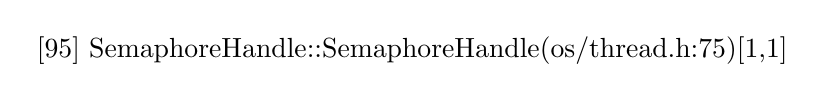
\begin{tikzpicture}[grow via three points={one child at (0.5,-0.7) and two children at (0.5,-0.7) and (0.5,-1.4)}, edge from parent path={(\tikzparentnode.south) |- (\tikzchildnode.west)}]
\node {[95] SemaphoreHandle::SemaphoreHandle(os/thread.h:75)[1,1]}
;
\end{tikzpicture}

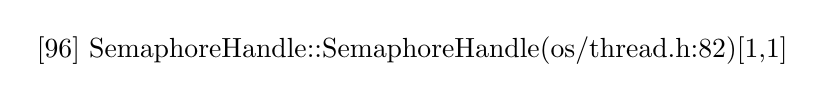
\begin{tikzpicture}[grow via three points={one child at (0.5,-0.7) and two children at (0.5,-0.7) and (0.5,-1.4)}, edge from parent path={(\tikzparentnode.south) |- (\tikzchildnode.west)}]
\node {[96] SemaphoreHandle::SemaphoreHandle(os/thread.h:82)[1,1]}
;
\end{tikzpicture}

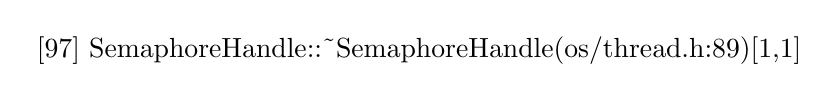
\begin{tikzpicture}[grow via three points={one child at (0.5,-0.7) and two children at (0.5,-0.7) and (0.5,-1.4)}, edge from parent path={(\tikzparentnode.south) |- (\tikzchildnode.west)}]
\node {[97] SemaphoreHandle::\~{}SemaphoreHandle(os/thread.h:89)[1,1]}
;
\end{tikzpicture}

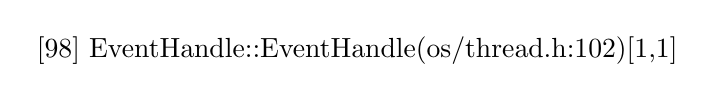
\begin{tikzpicture}[grow via three points={one child at (0.5,-0.7) and two children at (0.5,-0.7) and (0.5,-1.4)}, edge from parent path={(\tikzparentnode.south) |- (\tikzchildnode.west)}]
\node {[98] EventHandle::EventHandle(os/thread.h:102)[1,1]}
;
\end{tikzpicture}

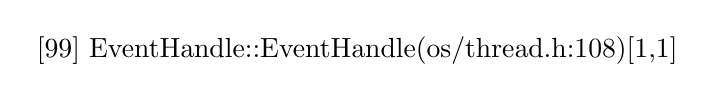
\begin{tikzpicture}[grow via three points={one child at (0.5,-0.7) and two children at (0.5,-0.7) and (0.5,-1.4)}, edge from parent path={(\tikzparentnode.south) |- (\tikzchildnode.west)}]
\node {[99] EventHandle::EventHandle(os/thread.h:108)[1,1]}
;
\end{tikzpicture}

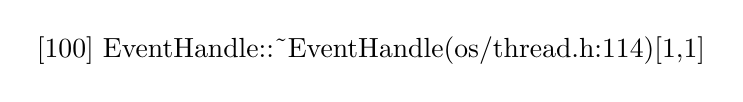
\begin{tikzpicture}[grow via three points={one child at (0.5,-0.7) and two children at (0.5,-0.7) and (0.5,-1.4)}, edge from parent path={(\tikzparentnode.south) |- (\tikzchildnode.west)}]
\node {[100] EventHandle::\~{}EventHandle(os/thread.h:114)[1,1]}
;
\end{tikzpicture}

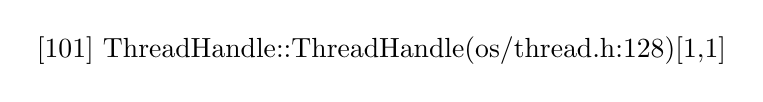
\begin{tikzpicture}[grow via three points={one child at (0.5,-0.7) and two children at (0.5,-0.7) and (0.5,-1.4)}, edge from parent path={(\tikzparentnode.south) |- (\tikzchildnode.west)}]
\node {[101] ThreadHandle::ThreadHandle(os/thread.h:128)[1,1]}
;
\end{tikzpicture}

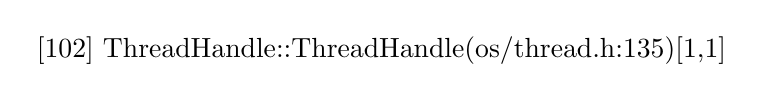
\begin{tikzpicture}[grow via three points={one child at (0.5,-0.7) and two children at (0.5,-0.7) and (0.5,-1.4)}, edge from parent path={(\tikzparentnode.south) |- (\tikzchildnode.west)}]
\node {[102] ThreadHandle::ThreadHandle(os/thread.h:135)[1,1]}
;
\end{tikzpicture}

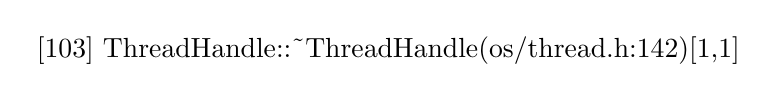
\begin{tikzpicture}[grow via three points={one child at (0.5,-0.7) and two children at (0.5,-0.7) and (0.5,-1.4)}, edge from parent path={(\tikzparentnode.south) |- (\tikzchildnode.west)}]
\node {[103] ThreadHandle::\~{}ThreadHandle(os/thread.h:142)[1,1]}
;
\end{tikzpicture}

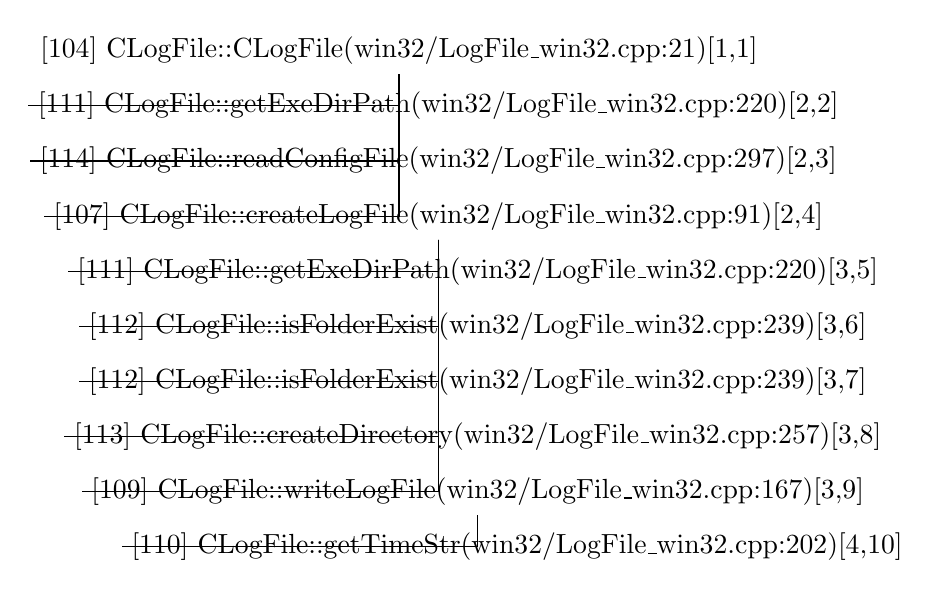
\begin{tikzpicture}[grow via three points={one child at (0.5,-0.7) and two children at (0.5,-0.7) and (0.5,-1.4)}, edge from parent path={(\tikzparentnode.south) |- (\tikzchildnode.west)}]
\node {[104] CLogFile::CLogFile(win32/LogFile\_win32.cpp:21)[1,1]}
    child { node {[111] CLogFile::getExeDirPath(win32/LogFile\_win32.cpp:220)[2,2]} 
        }
    child { node {[114] CLogFile::readConfigFile(win32/LogFile\_win32.cpp:297)[2,3]} 
        }
    child { node {[107] CLogFile::createLogFile(win32/LogFile\_win32.cpp:91)[2,4]} 
        child { node {[111] CLogFile::getExeDirPath(win32/LogFile\_win32.cpp:220)[3,5]} 
            }
        child { node {[112] CLogFile::isFolderExist(win32/LogFile\_win32.cpp:239)[3,6]} 
            }
        child { node {[112] CLogFile::isFolderExist(win32/LogFile\_win32.cpp:239)[3,7]} 
            }
        child { node {[113] CLogFile::createDirectory(win32/LogFile\_win32.cpp:257)[3,8]} 
            }
        child { node {[109] CLogFile::writeLogFile(win32/LogFile\_win32.cpp:167)[3,9]} 
            child { node {[110] CLogFile::getTimeStr(win32/LogFile\_win32.cpp:202)[4,10]} 
                }
            }
            child [missing] {}
            }
            child [missing] {}
            child [missing] {}
            child [missing] {}
            child [missing] {}
            child [missing] {}
            child [missing] {}
;
\end{tikzpicture}

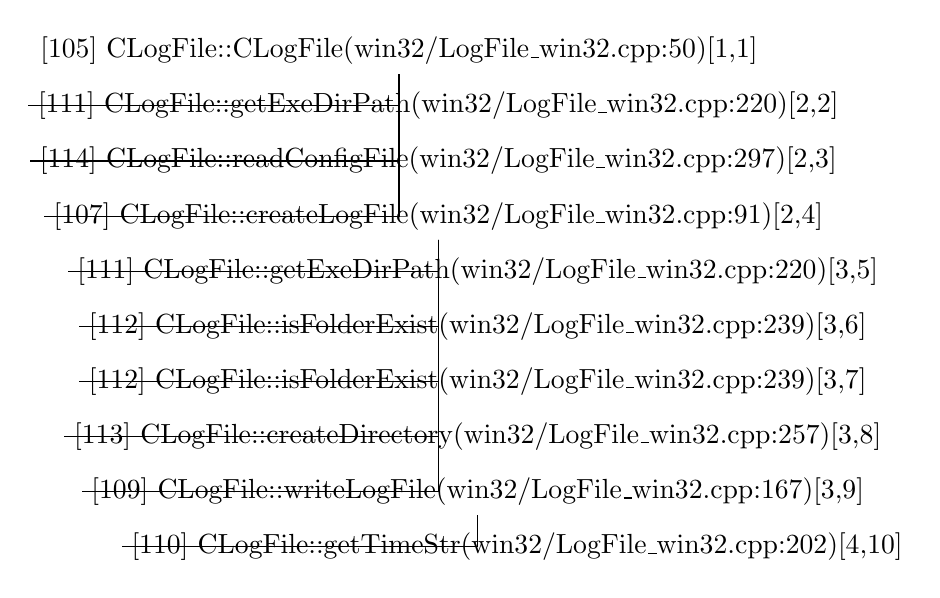
\begin{tikzpicture}[grow via three points={one child at (0.5,-0.7) and two children at (0.5,-0.7) and (0.5,-1.4)}, edge from parent path={(\tikzparentnode.south) |- (\tikzchildnode.west)}]
\node {[105] CLogFile::CLogFile(win32/LogFile\_win32.cpp:50)[1,1]}
    child { node {[111] CLogFile::getExeDirPath(win32/LogFile\_win32.cpp:220)[2,2]} 
        }
    child { node {[114] CLogFile::readConfigFile(win32/LogFile\_win32.cpp:297)[2,3]} 
        }
    child { node {[107] CLogFile::createLogFile(win32/LogFile\_win32.cpp:91)[2,4]} 
        child { node {[111] CLogFile::getExeDirPath(win32/LogFile\_win32.cpp:220)[3,5]} 
            }
        child { node {[112] CLogFile::isFolderExist(win32/LogFile\_win32.cpp:239)[3,6]} 
            }
        child { node {[112] CLogFile::isFolderExist(win32/LogFile\_win32.cpp:239)[3,7]} 
            }
        child { node {[113] CLogFile::createDirectory(win32/LogFile\_win32.cpp:257)[3,8]} 
            }
        child { node {[109] CLogFile::writeLogFile(win32/LogFile\_win32.cpp:167)[3,9]} 
            child { node {[110] CLogFile::getTimeStr(win32/LogFile\_win32.cpp:202)[4,10]} 
                }
            }
            child [missing] {}
            }
            child [missing] {}
            child [missing] {}
            child [missing] {}
            child [missing] {}
            child [missing] {}
            child [missing] {}
;
\end{tikzpicture}

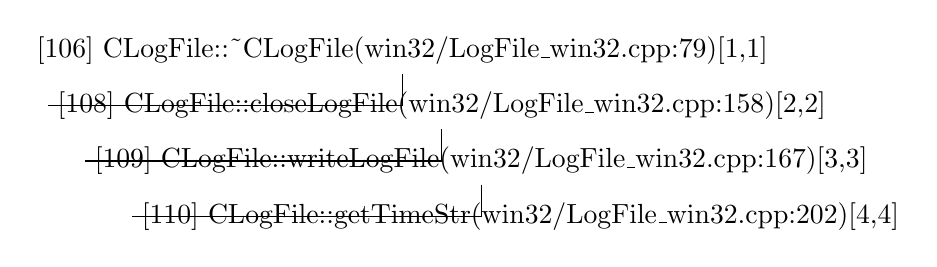
\begin{tikzpicture}[grow via three points={one child at (0.5,-0.7) and two children at (0.5,-0.7) and (0.5,-1.4)}, edge from parent path={(\tikzparentnode.south) |- (\tikzchildnode.west)}]
\node {[106] CLogFile::\~{}CLogFile(win32/LogFile\_win32.cpp:79)[1,1]}
    child { node {[108] CLogFile::closeLogFile(win32/LogFile\_win32.cpp:158)[2,2]} 
        child { node {[109] CLogFile::writeLogFile(win32/LogFile\_win32.cpp:167)[3,3]} 
            child { node {[110] CLogFile::getTimeStr(win32/LogFile\_win32.cpp:202)[4,4]} 
                }
            }
            child [missing] {}
            }
            child [missing] {}
            child [missing] {}
;
\end{tikzpicture}

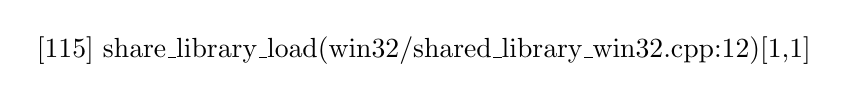
\begin{tikzpicture}[grow via three points={one child at (0.5,-0.7) and two children at (0.5,-0.7) and (0.5,-1.4)}, edge from parent path={(\tikzparentnode.south) |- (\tikzchildnode.west)}]
\node {[115] share\_library\_load(win32/shared\_library\_win32.cpp:12)[1,1]}
;
\end{tikzpicture}

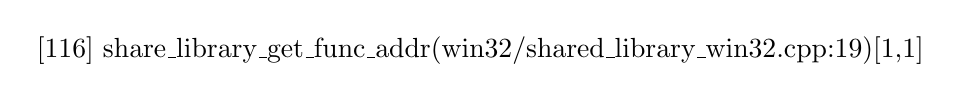
\begin{tikzpicture}[grow via three points={one child at (0.5,-0.7) and two children at (0.5,-0.7) and (0.5,-1.4)}, edge from parent path={(\tikzparentnode.south) |- (\tikzchildnode.west)}]
\node {[116] share\_library\_get\_func\_addr(win32/shared\_library\_win32.cpp:19)[1,1]}
;
\end{tikzpicture}

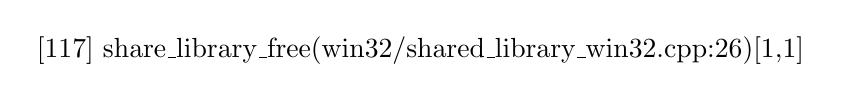
\begin{tikzpicture}[grow via three points={one child at (0.5,-0.7) and two children at (0.5,-0.7) and (0.5,-1.4)}, edge from parent path={(\tikzparentnode.south) |- (\tikzchildnode.west)}]
\node {[117] share\_library\_free(win32/shared\_library\_win32.cpp:26)[1,1]}
;
\end{tikzpicture}

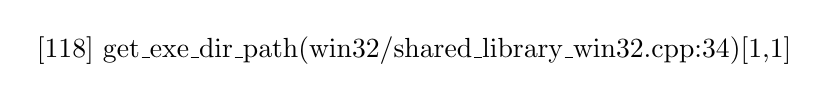
\begin{tikzpicture}[grow via three points={one child at (0.5,-0.7) and two children at (0.5,-0.7) and (0.5,-1.4)}, edge from parent path={(\tikzparentnode.south) |- (\tikzchildnode.west)}]
\node {[118] get\_exe\_dir\_path(win32/shared\_library\_win32.cpp:34)[1,1]}
;
\end{tikzpicture}

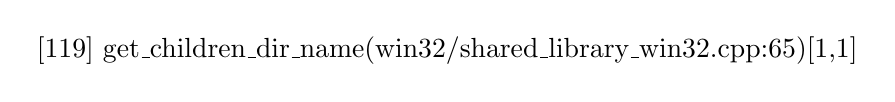
\begin{tikzpicture}[grow via three points={one child at (0.5,-0.7) and two children at (0.5,-0.7) and (0.5,-1.4)}, edge from parent path={(\tikzparentnode.south) |- (\tikzchildnode.west)}]
\node {[119] get\_children\_dir\_name(win32/shared\_library\_win32.cpp:65)[1,1]}
;
\end{tikzpicture}

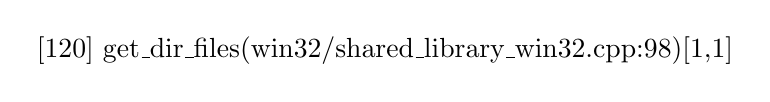
\begin{tikzpicture}[grow via three points={one child at (0.5,-0.7) and two children at (0.5,-0.7) and (0.5,-1.4)}, edge from parent path={(\tikzparentnode.south) |- (\tikzchildnode.west)}]
\node {[120] get\_dir\_files(win32/shared\_library\_win32.cpp:98)[1,1]}
;
\end{tikzpicture}

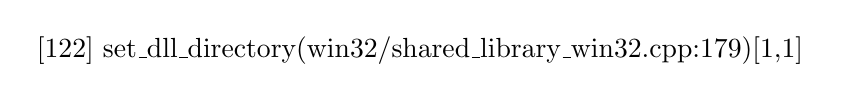
\begin{tikzpicture}[grow via three points={one child at (0.5,-0.7) and two children at (0.5,-0.7) and (0.5,-1.4)}, edge from parent path={(\tikzparentnode.south) |- (\tikzchildnode.west)}]
\node {[122] set\_dll\_directory(win32/shared\_library\_win32.cpp:179)[1,1]}
;
\end{tikzpicture}

\begin{tikzpicture}[grow via three points={one child at (0.5,-0.7) and two children at (0.5,-0.7) and (0.5,-1.4)}, edge from parent path={(\tikzparentnode.south) |- (\tikzchildnode.west)}]
\node {[123] is\_file\_exist(win32/shared\_library\_win32.cpp:186)[1,1]}
;
\end{tikzpicture}

\begin{tikzpicture}[grow via three points={one child at (0.5,-0.7) and two children at (0.5,-0.7) and (0.5,-1.4)}, edge from parent path={(\tikzparentnode.south) |- (\tikzchildnode.west)}]
\node {[124] print\_mem\_usage(win32/shared\_library\_win32.cpp:199)[1,1]}
;
\end{tikzpicture}

\begin{tikzpicture}[grow via three points={one child at (0.5,-0.7) and two children at (0.5,-0.7) and (0.5,-1.4)}, edge from parent path={(\tikzparentnode.south) |- (\tikzchildnode.west)}]
\node {[126] get\_current\_thread\_id(win32/shared\_library\_win32.cpp:238)[1,1]}
;
\end{tikzpicture}

\begin{tikzpicture}[grow via three points={one child at (0.5,-0.7) and two children at (0.5,-0.7) and (0.5,-1.4)}, edge from parent path={(\tikzparentnode.south) |- (\tikzchildnode.west)}]
\node {[127] create\_nested\_dir(win32/shared\_library\_win32.cpp:246)[1,1]}
;
\end{tikzpicture}

\begin{tikzpicture}[grow via three points={one child at (0.5,-0.7) and two children at (0.5,-0.7) and (0.5,-1.4)}, edge from parent path={(\tikzparentnode.south) |- (\tikzchildnode.west)}]
\node {[128] CMutex::CMutex(win32/thread\_win32.cpp:9)[1,1]}
;
\end{tikzpicture}

\begin{tikzpicture}[grow via three points={one child at (0.5,-0.7) and two children at (0.5,-0.7) and (0.5,-1.4)}, edge from parent path={(\tikzparentnode.south) |- (\tikzchildnode.west)}]
\node {[129] CMutex::\~{}CMutex(win32/thread\_win32.cpp:15)[1,1]}
    child { node {[131] CMutex::Unlock(win32/thread\_win32.cpp:29)[2,2]} 
        }
;
\end{tikzpicture}

\begin{tikzpicture}[grow via three points={one child at (0.5,-0.7) and two children at (0.5,-0.7) and (0.5,-1.4)}, edge from parent path={(\tikzparentnode.south) |- (\tikzchildnode.west)}]
\node {[133] CAutoMutex::\~{}CAutoMutex(win32/thread\_win32.cpp:50)[1,1]}
    child { node {[131] CMutex::Unlock(win32/thread\_win32.cpp:29)[2,2]} 
        }
;
\end{tikzpicture}

\begin{tikzpicture}[grow via three points={one child at (0.5,-0.7) and two children at (0.5,-0.7) and (0.5,-1.4)}, edge from parent path={(\tikzparentnode.south) |- (\tikzchildnode.west)}]
\node {[134] CAutoMutex::Lock(win32/thread\_win32.cpp:56)[1,1]}
    child { node {[132] CMutex::Try(win32/thread\_win32.cpp:36)[2,2]} 
        }
    child { node {[130] CMutex::Lock(win32/thread\_win32.cpp:22)[2,3]} 
        }
;
\end{tikzpicture}

\begin{tikzpicture}[grow via three points={one child at (0.5,-0.7) and two children at (0.5,-0.7) and (0.5,-1.4)}, edge from parent path={(\tikzparentnode.south) |- (\tikzchildnode.west)}]
\node {[135] CAutoMutex::Unlock(win32/thread\_win32.cpp:71)[1,1]}
    child { node {[131] CMutex::Unlock(win32/thread\_win32.cpp:29)[2,2]} 
        }
;
\end{tikzpicture}

\begin{tikzpicture}[grow via three points={one child at (0.5,-0.7) and two children at (0.5,-0.7) and (0.5,-1.4)}, edge from parent path={(\tikzparentnode.south) |- (\tikzchildnode.west)}]
\node {[136] CSemaphore::CSemaphore(win32/thread\_win32.cpp:84)[1,1]}
;
\end{tikzpicture}

\begin{tikzpicture}[grow via three points={one child at (0.5,-0.7) and two children at (0.5,-0.7) and (0.5,-1.4)}, edge from parent path={(\tikzparentnode.south) |- (\tikzchildnode.west)}]
\node {[137] CSemaphore::CSemaphore(win32/thread\_win32.cpp:90)[1,1]}
;
\end{tikzpicture}

\begin{tikzpicture}[grow via three points={one child at (0.5,-0.7) and two children at (0.5,-0.7) and (0.5,-1.4)}, edge from parent path={(\tikzparentnode.south) |- (\tikzchildnode.west)}]
\node {[138] CSemaphore::\~{}CSemaphore(win32/thread\_win32.cpp:98)[1,1]}
;
\end{tikzpicture}

\begin{tikzpicture}[grow via three points={one child at (0.5,-0.7) and two children at (0.5,-0.7) and (0.5,-1.4)}, edge from parent path={(\tikzparentnode.south) |- (\tikzchildnode.west)}]
\node {[139] CSemaphore::Post(win32/thread\_win32.cpp:104)[1,1]}
;
\end{tikzpicture}

\begin{tikzpicture}[grow via three points={one child at (0.5,-0.7) and two children at (0.5,-0.7) and (0.5,-1.4)}, edge from parent path={(\tikzparentnode.south) |- (\tikzchildnode.west)}]
\node {[140] CSemaphore::Wait(win32/thread\_win32.cpp:110)[1,1]}
;
\end{tikzpicture}

\begin{tikzpicture}[grow via three points={one child at (0.5,-0.7) and two children at (0.5,-0.7) and (0.5,-1.4)}, edge from parent path={(\tikzparentnode.south) |- (\tikzchildnode.west)}]
\node {[141] CEvent::CEvent(win32/thread\_win32.cpp:117)[1,1]}
;
\end{tikzpicture}

\begin{tikzpicture}[grow via three points={one child at (0.5,-0.7) and two children at (0.5,-0.7) and (0.5,-1.4)}, edge from parent path={(\tikzparentnode.south) |- (\tikzchildnode.west)}]
\node {[142] CEvent::CEvent(win32/thread\_win32.cpp:123)[1,1]}
;
\end{tikzpicture}

\begin{tikzpicture}[grow via three points={one child at (0.5,-0.7) and two children at (0.5,-0.7) and (0.5,-1.4)}, edge from parent path={(\tikzparentnode.south) |- (\tikzchildnode.west)}]
\node {[143] CEvent::\~{}CEvent(win32/thread\_win32.cpp:131)[1,1]}
    child { node {[145] CEvent::Signal(win32/thread\_win32.cpp:149)[2,2]} 
        }
;
\end{tikzpicture}

\begin{tikzpicture}[grow via three points={one child at (0.5,-0.7) and two children at (0.5,-0.7) and (0.5,-1.4)}, edge from parent path={(\tikzparentnode.south) |- (\tikzchildnode.west)}]
\node {[144] CEvent::Init(win32/thread\_win32.cpp:142)[1,1]}
;
\end{tikzpicture}

\begin{tikzpicture}[grow via three points={one child at (0.5,-0.7) and two children at (0.5,-0.7) and (0.5,-1.4)}, edge from parent path={(\tikzparentnode.south) |- (\tikzchildnode.west)}]
\node {[146] CEvent::Reset(win32/thread\_win32.cpp:155)[1,1]}
;
\end{tikzpicture}

\begin{tikzpicture}[grow via three points={one child at (0.5,-0.7) and two children at (0.5,-0.7) and (0.5,-1.4)}, edge from parent path={(\tikzparentnode.south) |- (\tikzchildnode.west)}]
\node {[147] CEvent::Wait(win32/thread\_win32.cpp:161)[1,1]}
;
\end{tikzpicture}

\begin{tikzpicture}[grow via three points={one child at (0.5,-0.7) and two children at (0.5,-0.7) and (0.5,-1.4)}, edge from parent path={(\tikzparentnode.south) |- (\tikzchildnode.west)}]
\node {[148] CEvent::TimedWait(win32/thread\_win32.cpp:167)[1,1]}
;
\end{tikzpicture}

\begin{tikzpicture}[grow via three points={one child at (0.5,-0.7) and two children at (0.5,-0.7) and (0.5,-1.4)}, edge from parent path={(\tikzparentnode.south) |- (\tikzchildnode.west)}]
\node {[149] CThread::CThread(win32/thread\_win32.cpp:189)[1,1]}
;
\end{tikzpicture}

\begin{tikzpicture}[grow via three points={one child at (0.5,-0.7) and two children at (0.5,-0.7) and (0.5,-1.4)}, edge from parent path={(\tikzparentnode.south) |- (\tikzchildnode.west)}]
\node {[150] CThread::CThread(win32/thread\_win32.cpp:199)[1,1]}
;
\end{tikzpicture}

\begin{tikzpicture}[grow via three points={one child at (0.5,-0.7) and two children at (0.5,-0.7) and (0.5,-1.4)}, edge from parent path={(\tikzparentnode.south) |- (\tikzchildnode.west)}]
\node {[151] CThread::\~{}CThread(win32/thread\_win32.cpp:212)[1,1]}
;
\end{tikzpicture}

\begin{tikzpicture}[grow via three points={one child at (0.5,-0.7) and two children at (0.5,-0.7) and (0.5,-1.4)}, edge from parent path={(\tikzparentnode.south) |- (\tikzchildnode.west)}]
\node {[152] CThread::Begin(win32/thread\_win32.cpp:222)[1,1]}
    child { node {[130] CMutex::Lock(win32/thread\_win32.cpp:22)[2,2]} 
        }
    child { node {[131] CMutex::Unlock(win32/thread\_win32.cpp:29)[2,3]} 
        }
;
\end{tikzpicture}

\begin{tikzpicture}[grow via three points={one child at (0.5,-0.7) and two children at (0.5,-0.7) and (0.5,-1.4)}, edge from parent path={(\tikzparentnode.south) |- (\tikzchildnode.west)}]
\node {[153] CThread::End(win32/thread\_win32.cpp:240)[1,1]}
;
\end{tikzpicture}

\begin{tikzpicture}[grow via three points={one child at (0.5,-0.7) and two children at (0.5,-0.7) and (0.5,-1.4)}, edge from parent path={(\tikzparentnode.south) |- (\tikzchildnode.west)}]
\node {[154] CThread::IsEnd(win32/thread\_win32.cpp:250)[1,1]}
;
\end{tikzpicture}

\begin{tikzpicture}[grow via three points={one child at (0.5,-0.7) and two children at (0.5,-0.7) and (0.5,-1.4)}, edge from parent path={(\tikzparentnode.south) |- (\tikzchildnode.west)}]
\node {[155] CThread::Dead(win32/thread\_win32.cpp:262)[1,1]}
;
\end{tikzpicture}

\begin{tikzpicture}[grow via three points={one child at (0.5,-0.7) and two children at (0.5,-0.7) and (0.5,-1.4)}, edge from parent path={(\tikzparentnode.south) |- (\tikzchildnode.west)}]
\node {[156] CThread::IsDead(win32/thread\_win32.cpp:269)[1,1]}
;
\end{tikzpicture}

\begin{tikzpicture}[grow via three points={one child at (0.5,-0.7) and two children at (0.5,-0.7) and (0.5,-1.4)}, edge from parent path={(\tikzparentnode.south) |- (\tikzchildnode.west)}]
\node {[157] CThread::Wait(win32/thread\_win32.cpp:275)[1,1]}
;
\end{tikzpicture}

\begin{tikzpicture}[grow via three points={one child at (0.5,-0.7) and two children at (0.5,-0.7) and (0.5,-1.4)}, edge from parent path={(\tikzparentnode.south) |- (\tikzchildnode.west)}]
\node {[158] CThread::TimedWait(win32/thread\_win32.cpp:281)[1,1]}
;
\end{tikzpicture}

\begin{tikzpicture}[grow via three points={one child at (0.5,-0.7) and two children at (0.5,-0.7) and (0.5,-1.4)}, edge from parent path={(\tikzparentnode.south) |- (\tikzchildnode.west)}]
\node {[159] CThread::GetExitCode(win32/thread\_win32.cpp:303)[1,1]}
;
\end{tikzpicture}

\begin{tikzpicture}[grow via three points={one child at (0.5,-0.7) and two children at (0.5,-0.7) and (0.5,-1.4)}, edge from parent path={(\tikzparentnode.south) |- (\tikzchildnode.west)}]
\node {[160] CThread::GetThreadId(win32/thread\_win32.cpp:326)[1,1]}
;
\end{tikzpicture}

\begin{tikzpicture}[grow via three points={one child at (0.5,-0.7) and two children at (0.5,-0.7) and (0.5,-1.4)}, edge from parent path={(\tikzparentnode.south) |- (\tikzchildnode.west)}]
\node {[161] CThread::Suspend(win32/thread\_win32.cpp:332)[1,1]}
    child { node {[130] CMutex::Lock(win32/thread\_win32.cpp:22)[2,2]} 
        }
    child { node {[131] CMutex::Unlock(win32/thread\_win32.cpp:29)[2,3]} 
        }
;
\end{tikzpicture}

\begin{tikzpicture}[grow via three points={one child at (0.5,-0.7) and two children at (0.5,-0.7) and (0.5,-1.4)}, edge from parent path={(\tikzparentnode.south) |- (\tikzchildnode.west)}]
\node {[162] CThread::Resume(win32/thread\_win32.cpp:346)[1,1]}
    child { node {[130] CMutex::Lock(win32/thread\_win32.cpp:22)[2,2]} 
        }
    child { node {[131] CMutex::Unlock(win32/thread\_win32.cpp:29)[2,3]} 
        }
    child { node {[145] CEvent::Signal(win32/thread\_win32.cpp:149)[2,4]} 
        }
;
\end{tikzpicture}

\begin{tikzpicture}[grow via three points={one child at (0.5,-0.7) and two children at (0.5,-0.7) and (0.5,-1.4)}, edge from parent path={(\tikzparentnode.south) |- (\tikzchildnode.west)}]
\node {[163] CThread::IsSuspended(win32/thread\_win32.cpp:362)[1,1]}
;
\end{tikzpicture}

\begin{tikzpicture}[grow via three points={one child at (0.5,-0.7) and two children at (0.5,-0.7) and (0.5,-1.4)}, edge from parent path={(\tikzparentnode.south) |- (\tikzchildnode.west)}]
\node {[164] atomic\_inc16(win32/thread\_win32.cpp:380)[1,1]}
;
\end{tikzpicture}

\begin{tikzpicture}[grow via three points={one child at (0.5,-0.7) and two children at (0.5,-0.7) and (0.5,-1.4)}, edge from parent path={(\tikzparentnode.south) |- (\tikzchildnode.west)}]
\node {[165] atomic\_dec16(win32/thread\_win32.cpp:386)[1,1]}
;
\end{tikzpicture}

\begin{tikzpicture}[grow via three points={one child at (0.5,-0.7) and two children at (0.5,-0.7) and (0.5,-1.4)}, edge from parent path={(\tikzparentnode.south) |- (\tikzchildnode.west)}]
\node {[168] rdtsc(win32/timer\_win32.cpp:24)[1,1]}
;
\end{tikzpicture}

\end{document}
